\documentclass[a4paper,twoside, openright,12pt]{report}
\usepackage{psfrag,amsbsy,graphics,float}
\usepackage[dvips]{graphicx, color}
\usepackage[latin1]{inputenc}
\usepackage{verbatim} 
\usepackage{appendix}
\usepackage{amsmath}
\usepackage{subfigure}
% MY CHANGE
%\usepackage[bookmarksnumbered=true]{hyperref} 

\usepackage[bookmarks=true,colorlinks=true,       % false: boxed links; true: colored links
    linkcolor=black,          % color of internal links
    citecolor=black,        % color of links to bibliography
    filecolor=black,      % color of file links
    urlcolor=black           % color of external links
]{hyperref}
 

%%% Stand 14.09.2007
%%% erstellt von Marion Sobotka
%%% marion.sobotka@tum.de
%%% last changes: 14.01.09


%_______Kopf- und Fu�zeile_______________________________________________________
\usepackage{fancyhdr}
\pagestyle{fancy}
%um Kopf- und Fu�zeile bei chapter-Seiten zu reaktivieren
\newcommand{\helv}{%
   \fontfamily{phv}\fontseries{a}\fontsize{9}{11}\selectfont}
\fancypagestyle{plain}{	
	\fancyfoot{}% keine Fu�zeile
	\fancyhead[RE]{\helv\leftmark}% Rechts auf geraden Seiten=innen; in \leftmark stehen \chapters
	\fancyhead[LO]{\helv\rightmark}% Links auf ungeraden Seiten=au�en;in \rightmark stehen \sections
	\fancyhead[RO,LE]{\thepage}}%Rechts auf ungeraden und links auf geraden Seiten
%Kopf- und Fu�zeile f�r alle anderen Seiten
\fancyfoot{}
\fancyhead[RE]{\helv\leftmark}
\fancyhead[LO]{\helv\rightmark}%alt:\fancyhead[LO]{\itshape\rightmark}
\fancyhead[RO,LE]{\thepage}
%________________________________________________________________________________


%_Definieren der R�nder und L�ngen__________
\setlength{\textwidth}{15cm}
\setlength{\textheight}{22cm}
\setlength{\evensidemargin}{-2mm}
\setlength{\oddsidemargin}{11mm}
\setlength{\headwidth}{15cm}
\setlength{\topmargin}{10mm}
\setlength{\parindent}{0pt} % Kein Einr�cken beim Absatz!!
%___________________________________________


%_______Titelseite__________________________________________
\begin{document}
\pagestyle{empty}
\enlargethispage{4.5cm} %Damit das Titelbild weit genug unten ist!
\begin{center}
\phantom{u}
\vspace{0.5cm}
\Huge{\sc Numerical Test Rig for Large-Scale and Interconnected Dynamical
Systems}\\
\vspace{1.5cm}
                                 \large{submitted\\
				  Project Laboratory\\
				  Networked and Cooperative Control\\
			  %DIPLOMARBEIT\\%/STUDIENARBEIT/MASTERRBEIT/BACHELORARBEIT\\ 
                               %            von\\
                              %  \large{Zwischenbericht zur\\
			%DIPLOMARBEIT/STUDIENARBEIT/MASTERARBEIT/
					   % BACHELORARBEIT\\ 
					   by         

						
					\begin{tabular}{c c}
					    \vspace{0.4cm} & \vspace{0.4cm} \\
					 cand. ing. Francisco Llobet& cand. ing. Jose Rivera  \\
						\vspace{0.5cm} & \vspace{0.5cm}\\
					born on July 9, 1985 & born on December 18, 1986\\
					resident: & resident:\\
					Briennerstr. 39& Amalienstr. 87\\
					80333 M\"{u}nchen & 80799 M\"{u}nchen  
					\end{tabular}

					                           
					%Tel.: +49\,176\,233\,14721\\
					\vspace{1.5cm}
					Institute of\\
					Automatic Control Engineering\\
					Technische Universit\"{a}t M\"{u}nchen\\
					\vspace{0.3cm}
					Univ.-Prof. Dr.-Ing./Univ. Tokio Martin Buss\\
                                        Univ.-Prof. Dr.-Ing. Sandra Hirche}
\end{center}
\vspace{2.5cm}
\begin{tabular}{ll}
Supervisor: & F. Deroo, S. Erhart, A. Gusrialdi, H. Mangesius  \\
Beginn: & 09.05.2011  \\
Submitted &  04.07.2011 \\
\end{tabular}
%____________________________________________________________

\newpage

%_______Abstract_____________________________________________
\topmargin5mm
\textheight220mm
\pagenumbering{arabic}
\phantom{u}
\begin{abstract}
The goal of this project was to develop a test rig for large-scale and interconnected dynamical systems. The result is
MTIDS or Matlab Toolbox for Interconnected Dynamical Systems, which is a mash-up that wraps different toolboxes used for graph analysis and 
dynamic systems simulation together. MTIDS allows the definition and analysis of graphs, where each node has a specific dynamic assign to it. 
The template based design of nodes' dynamics allows great flexibility for the creation of complex interconnected dynamical systems with the 
possibility of implementing clusters/layers. MTIDS is an open-source project under the GNU GPL v2 license. This document presents a general description 
of MTIDS and instructions for its use.    
\vspace{2cm}
\begin{center}
\normalsize \textbf{Zusammenfassung}\\
\end{center}
Ziel dieses Projektes war es, eine Testvorrichtung f\"{u}r grosse, gekoppelte dynamische Systeme zu entwickeln. Das Ergebnis ist 
MTIDS oder Matlab Toolbox for Interconnected Dynamical
Systems. Diese Toolbox verbindet Toolboxen f\"{u}r die Graphenanalyse mit Toolboxen f\"{u}r die Simulation von dynamischen Systemen. 
MTIDS erm\"{o}glicht die Definition und Analyse von Graphen, bei denen jeder Knoten eine spezifische dynamische Anweisung ausf\"{u}hrt. 
Das Template basierte Design der Knotendynamik erlaubt eine gro\ss{}e Flexibilit\"{a}t f\"{u}r die Erstellung von komplexen, gekoppelten dynamischen Systemen. 
Es besteht beispielsweise die M\"{o}glichkeit Cluster bzw. Layer zu implementieren. MIDS ist ein Open-Source-Projekt unter der GNU GPL v2 Lizenz. 
Im Rahmen des nachfolgenden Berichts wird eine generelle Beschreibung von MTIDS sowie deren Benutzung gegeben.
\end{abstract}
%____________________________________________________________

\newpage

%_______Widmung_______________________________________________
\phantom{u}
\phantom{1}\vspace{6cm}
\begin{center}
%Hier die Widmung oder leer lassen
\end{center}
%_____________________________________________________________



\pagestyle{fancy}

%_________Inhaltsverzeichnis__________________________
\tableofcontents 
%_____________________________________________________




%_________Einleitung__________________________________
\chapter{Introduction} \label{chapter1}

In this first Chapter the motivation behind the MTIDS project is explained and the project's goal and framework is presented.

\section{Motivation}
Large-scale interconnected dynamical system are everywhere: biological systems, power and water distribution systems, the brain, 
social interaction networks, economic markets, etc. In a canonical form all of this systems can be thought as a bunch of nodes with local dynamics 
that interact with each other, e.g. a graph. Different topologies of the graph, may lead to different behavior. An example of various 
large scale interconnected systems can be seen in Figure \ref{largePic}. 


\begin{figure}[htb]
\centering
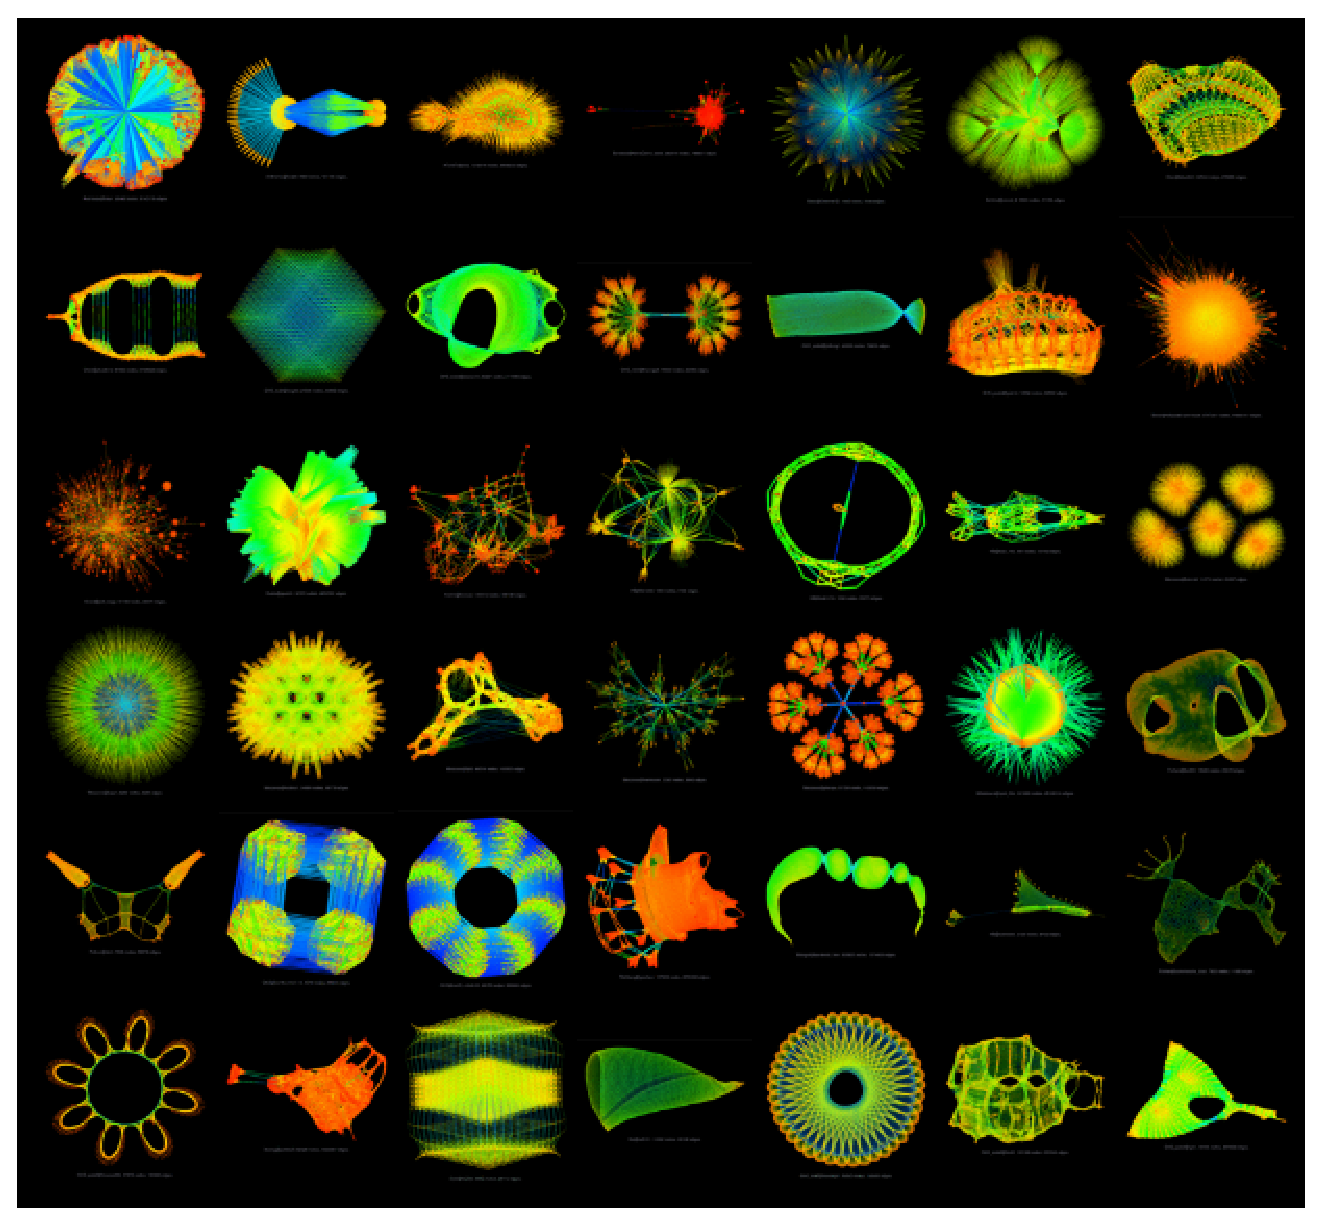
\includegraphics[width=0.5\textwidth]{pics/complex.eps}
\caption[Example of large-scale systems]{Visualization of various large scale systems using the sfdp algorithm $\copyright$ Dr. Yifan Hu of AT\&T Labs}
\label{largePic}
\end{figure}

There are many tools available for the analysis of interconnected dynamical systems, for example, in power systems you have PSSE and Power Factory. However,
this simulation programs are normally very system specific and in most cases it takes a long time to learn how to use them correctly. 
The difficulties are specially noticed while
testing control concepts, where small changes on the topology of the grid or control concept could lead to a painful redesign of your simulation set up. 
You may actually end up spending the most of your time in the implementation of a simulation. A more general and 
easy to use solution for the simulation of interconnected dynamical systems is needed.




\section{Idea and Goal}

\textbf{MTIDS} (Matlab Toolbox for Interconnected Dynamical Systems) is a project that aims to design an easy 
to use and flexible toolbox to make the simulation of large scale dynamical systems easier for students and researchers. 
The \textbf{goal} is to produce a mash-up that wraps different toolboxes used for graph analysis and 
dynamic systems simulation together into a framework.  


\begin{figure}[htb]
\centering
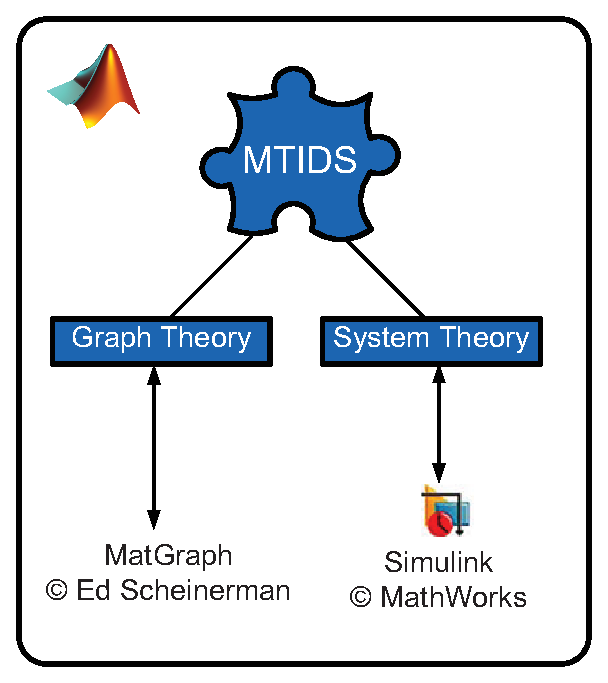
\includegraphics[width=0.5\textwidth]{pics/mtidsStructure.eps}
\caption[MTIDS idea]{MTIDS: Matlab Toolbox for Interconnected Dynamical Systems}
\label{mtidsFig}
\end{figure}

As we can see in Figure \ref{mtidsFig} MTIDS runs in the MATLAB environment and is basically a GUI that allows the interaction of tools used in graph theory 
and control theory.  For graph theory we use Matgraph a toolbox design by Prof. Scheinerman of the John Hopkins University \cite{MatgraphByExample} and for dynamical simulations
we use Simulink\cite{MatlabDocu}. 

\section{Framework}

The current framework of MTID is made out of three basic components. A GUI (\textbf{mtids.m}) an export to simulink function (\textbf{exportSimulink.m}) and
an import from Simulink function (\textbf{importSimulink.m}).\\

 

\begin{figure}[htb]
\centering
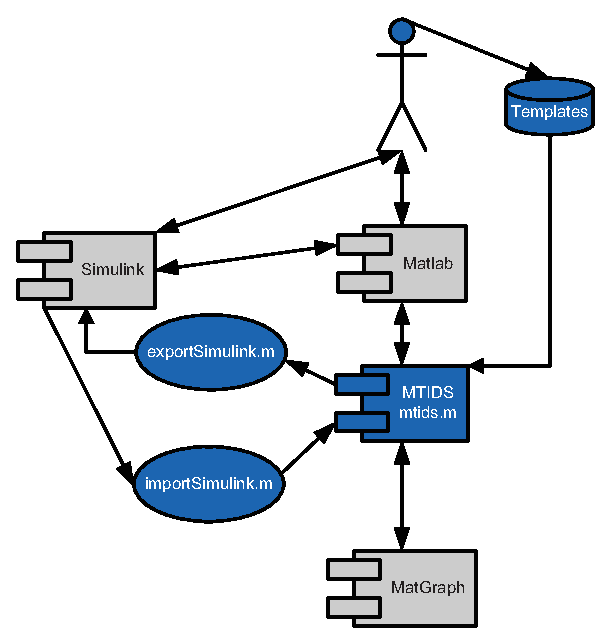
\includegraphics[width=0.5\textwidth]{pics/uml.eps}
\caption[MTIDS components]{MTIDS: Components diagram}
\label{componentsFig}
\end{figure}

In Figure \ref{componentsFig} we can see that the most important component is the user, specially its head. The better you are at producing templates
and interacting with Matlab and Simulation the more functional MTIDS is going to be for you.
In a nutshell MTIDS works as follows:
\begin{itemize}
\item GUI (mtids.m) runs inside Matlab.
\item GUI interacts with Matgraph: create, modify and visualize graphs.  
\item System Inteconnector (SI): exportSimulink.m and importSimulink.m called from GUI to interact with Simulink.
\item Templates done by User in Matlab/Simulink.
\item Simulations done in Simulink.
\end{itemize}
%  
% 
% The GUI (mtids.m) runs inside matlab. The UI interacts 
% with Matgraph to create, modify and visualize graphs. The ystem Inteconnector (SI) compose of the functions exportSimulink.m and importSimulink.m are
% called from GUI to interact with Simulink. The user can define the nodes dynamic by building custom templates in Matlab/Simulink. The simulations are
% ultimately done in Simulink.

%%%%%%%%%%%%%%%%%%%%%%%%%%%%%%%%%%%%%%%%%%%%%%%%%%%%%% GRAPH
\chapter{Graph Theory}\label{chapter2}
 
%References for this chapter can be found at \cite{NCS}, \cite{Estrada}, \cite{HivePlots}

\section{Algebraic Graph Theory}

Graphs are an easy way of representing networked structures. A graph consists of: 
\begin{enumerate}
\item \textbf{Vertices:} Represent nodes, dynamical subsystems and/or agents.
\item \textbf{Edges:} Represent connections, links or couplings between vertices.
\end{enumerate}

\textbf{In this project, we consider only simple, undirected and unweighted graphs.} \linebreak

Algebraic graph theory describes graph properties using numbers (like invariants) and equations.
It is important first, to convert the graphical representation of a graph into a mathematically sound description like
matrices. Once a the corresponding matrices (like the Laplacian or adjacency matrices) have been derived, we can calculate it's properties \cite{NCS} 

The use of linear algebraic tools like rank, eigenvalue and eigenvector extraction of graph matrices is called \textit{Spectral Graph Theory} 

\subsubsection{Degree of a vertex and degree vector}
The degree of a vertex is the number of edges that are connected to it.
The vector whose i-th component is the degree of the i-th vertex is the degree vector $\vec{d}$. 
The degree vector can analysed using basic statistical tools for for mean, variance, min, max, span, etc.

\subsubsection{Graph heterogenity}
Graph heterogenity is the quotient between the standard deviation of the degree vector $\vec{d}$ and the mean of the degree vector.
\begin{equation}
 H = \frac{\sqrt{ var(\vec{d}) }}{\bar{\vec{d}}} 
\end{equation}
It describes the heterogenity between the connections to the nodes.   

\subsubsection{Maximal number of edges and graph density}
A complete graph is a graph where every vertex is connected to every other vertex. 
The number of vertices inside a complete graph is:
\begin{equation}
 N_{e_{MAX}} = \frac{1}{2} N_v \left( N_v - 1  \right)
\end{equation}  
Alternatively:
\begin{equation}
 N_{e_{MAX}} = \frac{1}{2} \left( {N_v^2 - N_v } \right)
\end{equation}  
Graph density is a number which describes the \textit{completeness} of a graph. It is defined as the
quotient between the actual number of edges $N_e$ and number of edges of a complete graph $N_{e_{MAX}}$ with the same number of vertices: 
\begin{equation}
 D = \frac{N_e}{N_{e_{MAX}}}
\end{equation} 

\begin{equation}
 D = 2\frac{N_e}{N_v^2 - N_v}
\end{equation} 

\subsection{Graph matrices}
\subsubsection{Adjacency Matrix}
The adjacency matrix is defined as a $N_v$ x $N_v$ matrix whose $(A)_{ij}$ component is equal to one if there is a connection between vertex $i$ and vertex $j$ or zero if not.

\subsubsection{Degree Matrix}
A degree matrix is a diagonal matrix whose diagonal $(D)_{ii}$ components are equal to the degree of the i-th vertex.
All other components for $(D)_{ij}$ $i \ne j$ are zero.

\begin{equation}
  (D)_{ij} = \left\{ \begin{array}{ll}
0  & \mbox{if $i \ne j$} \\
N_v(i) & \mbox{if $i = j$}
                \end{array} \right. 
\end{equation}


\subsubsection{Laplacian Matrix}
The Laplacian matrix is defined as the degree matrix $D$ minus the adjacency matrix $A$:
\begin{equation}
 L = D - A
\end{equation} 
The Laplacian matrix is used to characterize the algebraic connectivity of a graph.

\subsection{Algebraic connectivity and Fiedler vector}
\subsubsection{Algebraic connectivity}
For sorted the sorted eigenvalues of the Laplacian matrix
$ \lambda_1 \leq \lambda_2 \leq \ldots \leq \lambda_{N_v} $
we define the algebraic connectivity as the first nonzero eigenvalue. It's corresponding eigenvector is the Fiedler vector.
The algebraic connectivity is a meassure of how connected a system is. For example, in the consensus problem, the algebraic connectivity describes the rate of convergence of the system to it's final state. 

\subsubsection{Number of connected subgraphs}
The multiplicity of the zero eigenvalue ot the Laplacian matrix is the number of connected subgraphs inside the system. This is also the rank of the nullspace of the Laplacian matrix
$Rank( {Null}(L)) $.
From the rank-nullity theorem of linear algebra we know that the rank of a matrix and the rank of it's nullspace add up to the number of collumns. Therefore for a square matrix, the rank of the nullspace can be calculated using:
 \begin{equation}
 Rank( {Null}(L) ) = Rank(L) - N_v
\end{equation} 
\vspace{10cm}
%\subsection{Estrada Index}
%
%The Estrada index of a vertex i is  \cite{Estrada}
%\begin{equation}
%E(i) = {(e^{A})_{ii}}
%\end{equation} 
%
%The Estrada index of an adjacency matrix is:
%\begin{equation}
%E(A) = tr(e^{A})
%\end{equation} 
\pagebreak 
\section{Creating and visualizing systems in MTIDS}
\subsection{MTIDS GUI Overview}
\begin{figure}[h!]
 \centering
 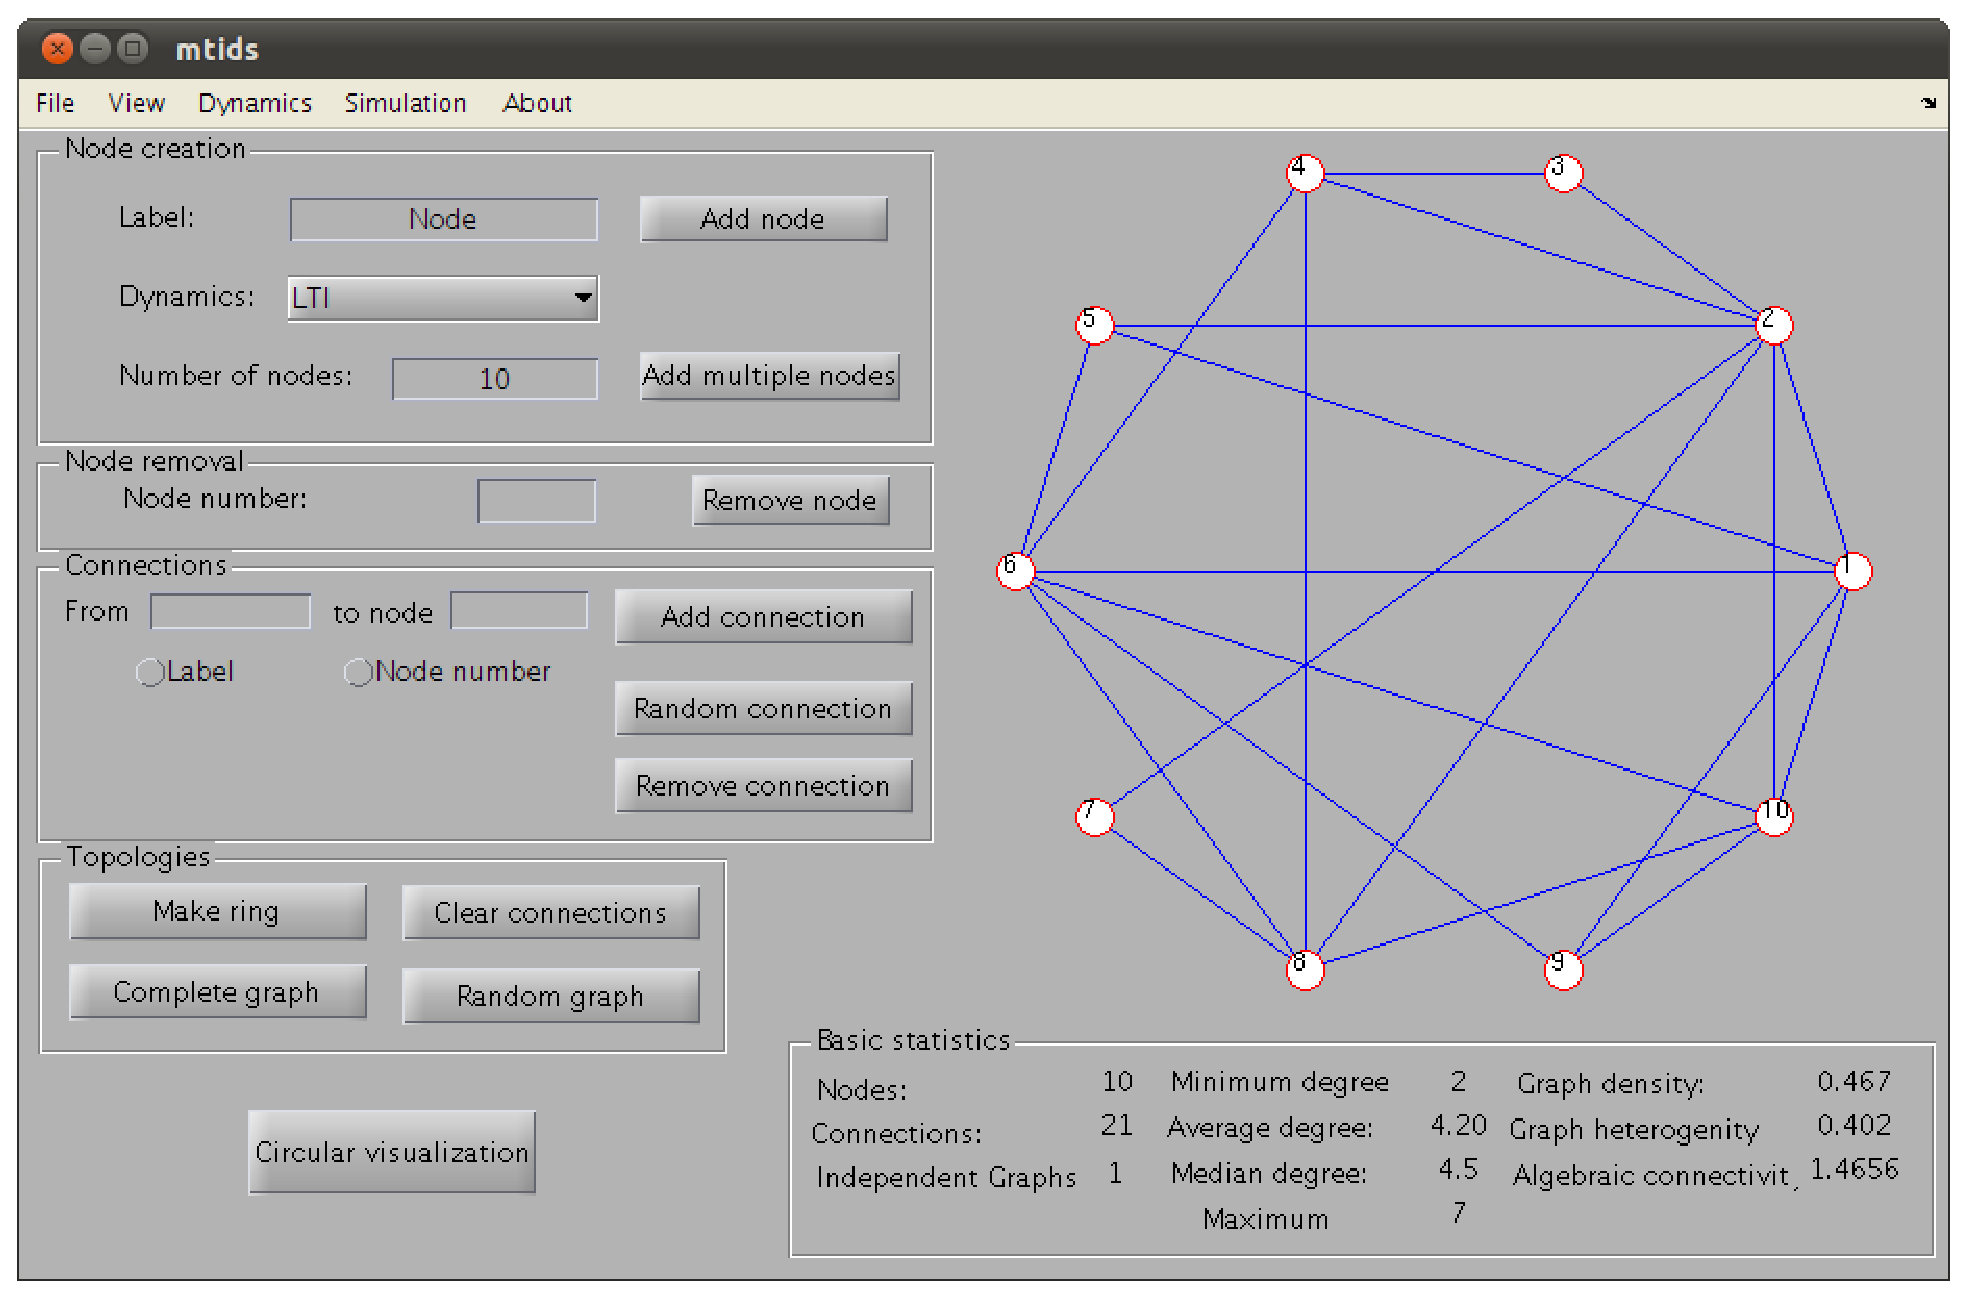
\includegraphics[width= \textwidth]{./pics/Mtits_UI.eps}
 % Mtits_UI.eps: 0x0 pixel, 300dpi, 0.00x0.00 cm, bb=14 14 943 621
 \caption{The MTIDS Graphical User Interface}
 \label{fig:MTIDS-UI}
\end{figure}
The MTIDS GUI is divided in two parts: The left side contains the controls that allow for modification of the system and the right side contains the graph and statistics visualization.

\subsection{Building an interconnected system in MTIDS}
\subsubsection{Adding nodes}
When adding a node, the User has to assign a unique node label and node dynamics at the ``node creation'' panel
Nodes can be added with the ``add node'' button or by (\verb|<Shift>-<Left-click>|) with the mouse.
Nodes added by using the mouse are given the last selected node dynamics and node label.

\subsubsection{Adding multiple nodes}
Adding multiple nodes at the same time is possible by introducing the number of nodes to be added and by clicking the ``Add multiple nodes'' button.
These nodes start all with the same name (eg. node1, node2,...) and share the same dynamics.
\subsubsection{Creating and removing connections}

Connections can be added or removed using:
\begin{itemize}
\item \textbf{Mouse:} By \verb|<Ctrl>-<Left click>| on both nodes. If no connection exists, it will create one, otherwise it will delete this connection. 
\item \textbf{Connection subwindow:} Connections to be added or removed can be specified by using node label or node number. 
\item \textbf{``Edit node'' dialog:} See Subsection \ref{node_properties}.
\end{itemize}

%\begin{figure}[h!]
% \centering
% 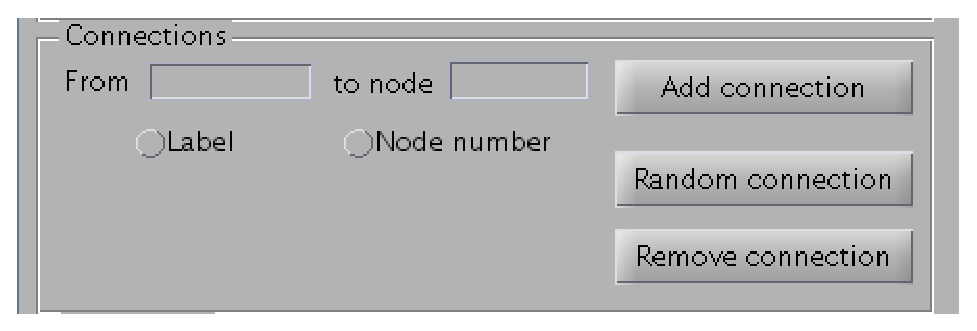
\includegraphics{./pics/mtids-ui-connections.eps}
% % mtids-ui-connections.eps: 0x0 pixel, 300dpi, 0.00x0.00 cm, bb=14 14 467 157
% \label{fig:mtids-ui-connections}
%\caption{Connection options}
%\end{figure}

Connections in MTIDS are bidirectional.

\subsubsection{Default topologies}

\begin{figure}[h!]
 \centering
 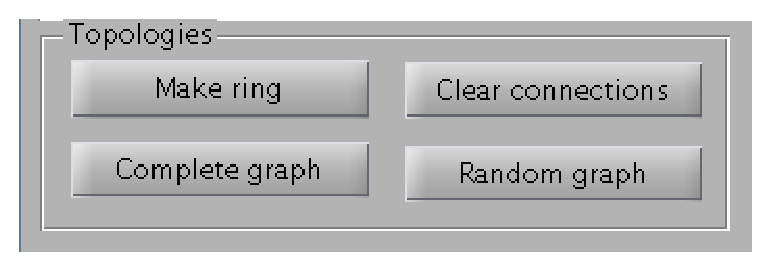
\includegraphics{./pics/mtids-ui-topologies.eps}
 % mtids-ui-topologies.eps: 0x0 pixel, 300dpi, 0.00x0.00 cm, bb=14 14 368 127
 \caption{The default topologies}
 \label{fig:mtids-ui-topologies}
\end{figure}

\begin{itemize}
\item \textbf{Complete graph:} Makes the graph into a complete graph.
\item \textbf{Remove connections:} Removes all edges inside the graph.
\item \textbf{Make ring:} Connects all nodes into a ring.
\item \textbf{Random graph:} Uses the random graph function from Matgraph. It adds random connections between nodes up to a density of ca. 0.5.
\end{itemize}

\subsection{Node properties}\label{node_properties}
\begin{figure}[h!]
 \centering
 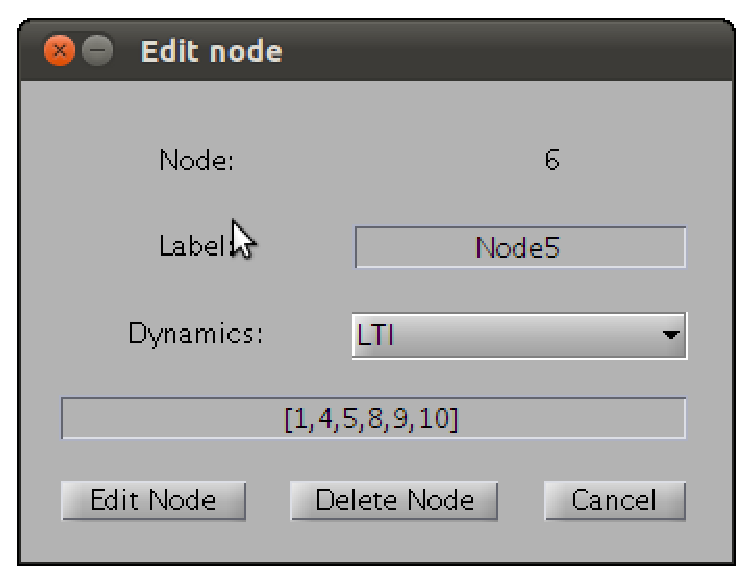
\includegraphics[width=0.6\textwidth]{./pics/Edit_node.eps}
 % Edit_node.eps: 0x0 pixel, 300dpi, 0.00x0.00 cm, bb=14 14 360 278
 \caption{The node properties window}
 \label{fig:Edit_Node}
\end{figure}
Node properties can be edited by \verb|<double-clicking>| a node in the graph window. 
Following node properties can be changed: Node label, node dynamics (from list) and the connection list vector in Matlab format.
The selected node can also be removed using this window.                         

\subsection{Load and Save}
A system can be saved by selecting \textbf{File $\rightarrow$ Save As...}. This saves the graph properties (adjacency matrix), node labels, assigned node dynamics and template list into a binary .mat file.
Loading an already saved system for modification is possible by selecting \textbf{File $\rightarrow$ Load...}. This loads the selected .mat file which contains the system properties. \linebreak
Remember that a saved system file contains the template names previously imported so reimporting dynamics is not necesary.
If a template .mdl file is missing or was deleted, the exporting to Simulink functionality will not work correctly.

\subsection{Exporting matrices to Matlab}
Select the corresponding workplace inside Matlab, variable name and matrix type to export.
Supported matrices are Laplacian matrix, adjacency matrix and edge list.

\subsection{Importing graph matrices into MTIDS}
Graph matrices like Laplacian matrix, adjacency matrix or edge list. The matrix type is automatically detected and replaces the current graph. Node dynamics are assigned based on the last selected template.
% End del graph Theory


%_%%%%%%%%%%%%%%%%%%%%%%%%%%%%%%%%%%%%%%%%%%%%%%%%%%%%%%%%%%%%%%%%%%%%%%%%%%%%%%%%%%%%%%%%%% SYSTEM_____________________________________
\chapter{System Theory}\label{chapter3}

In this Chapter we explain the design and simulation capabilities that MTIDS offers for interconnected dynamical systems.

\section{MTIDS Concepts for Simulink Models} \label{subsystemConcept}
MTIDS has two different concepts for building Simulink models. The difference relies on the amount of inputs that each node has.
\\

In the first concept, \textbf{concept 1}, each node has the same amount of inputs as there are nodes on the graph, even if the input is not connected. This concept is very efficient 
for matrix based description of system dynamics, where you describe the whole system at once,  like with LTI modeling.  \\

In \textbf{concept 2}, each node has only an input for the nodes that are connected to it. This is very efficient for agent or subsystem based descriptions, 
where the dynamics of each node may not allow a matrix based description of the  whole system. This concept is used for the examples of 
consensus and fireflies synchronization.     

\subsection{Nodes and connections}
\subsubsection{Node:}
Each node in MTIDS is a subsystem block in Simulink. Each node must have a unique label.
In \textbf{concept 1} each node has an in-port for every node in the graph and a single out-port. In \textbf{concept 2} each node has an in-port only 
for nodes connected to it and a single out-port.
\subsubsection{Connections:}
Any connection made inside MTIDS is bidirectional and unweighted. As Simulink connections are directed, each MTIDS bidirectional connection
 is represented with two directed connections between nodes. To implement weighted graphs, weights 
on branches have to be realized in the node's dynamic model, e.g inside the subsystem. Another option is to define junction nodes.

\section{Export to Simulink}\label{exportToSimulink}
In order to export the model created in the MTIDS GUI to simulink: \textbf{Simulation $\rightarrow$ Export to Simulink 1...} for  \textbf{concept 1} 
or \textbf{Simulation $\rightarrow$ Export to Simulink 2...} for \textbf{ concept 2} (see Figure \ref{exportFig}).
\\
\begin{figure}[htb]
\centering
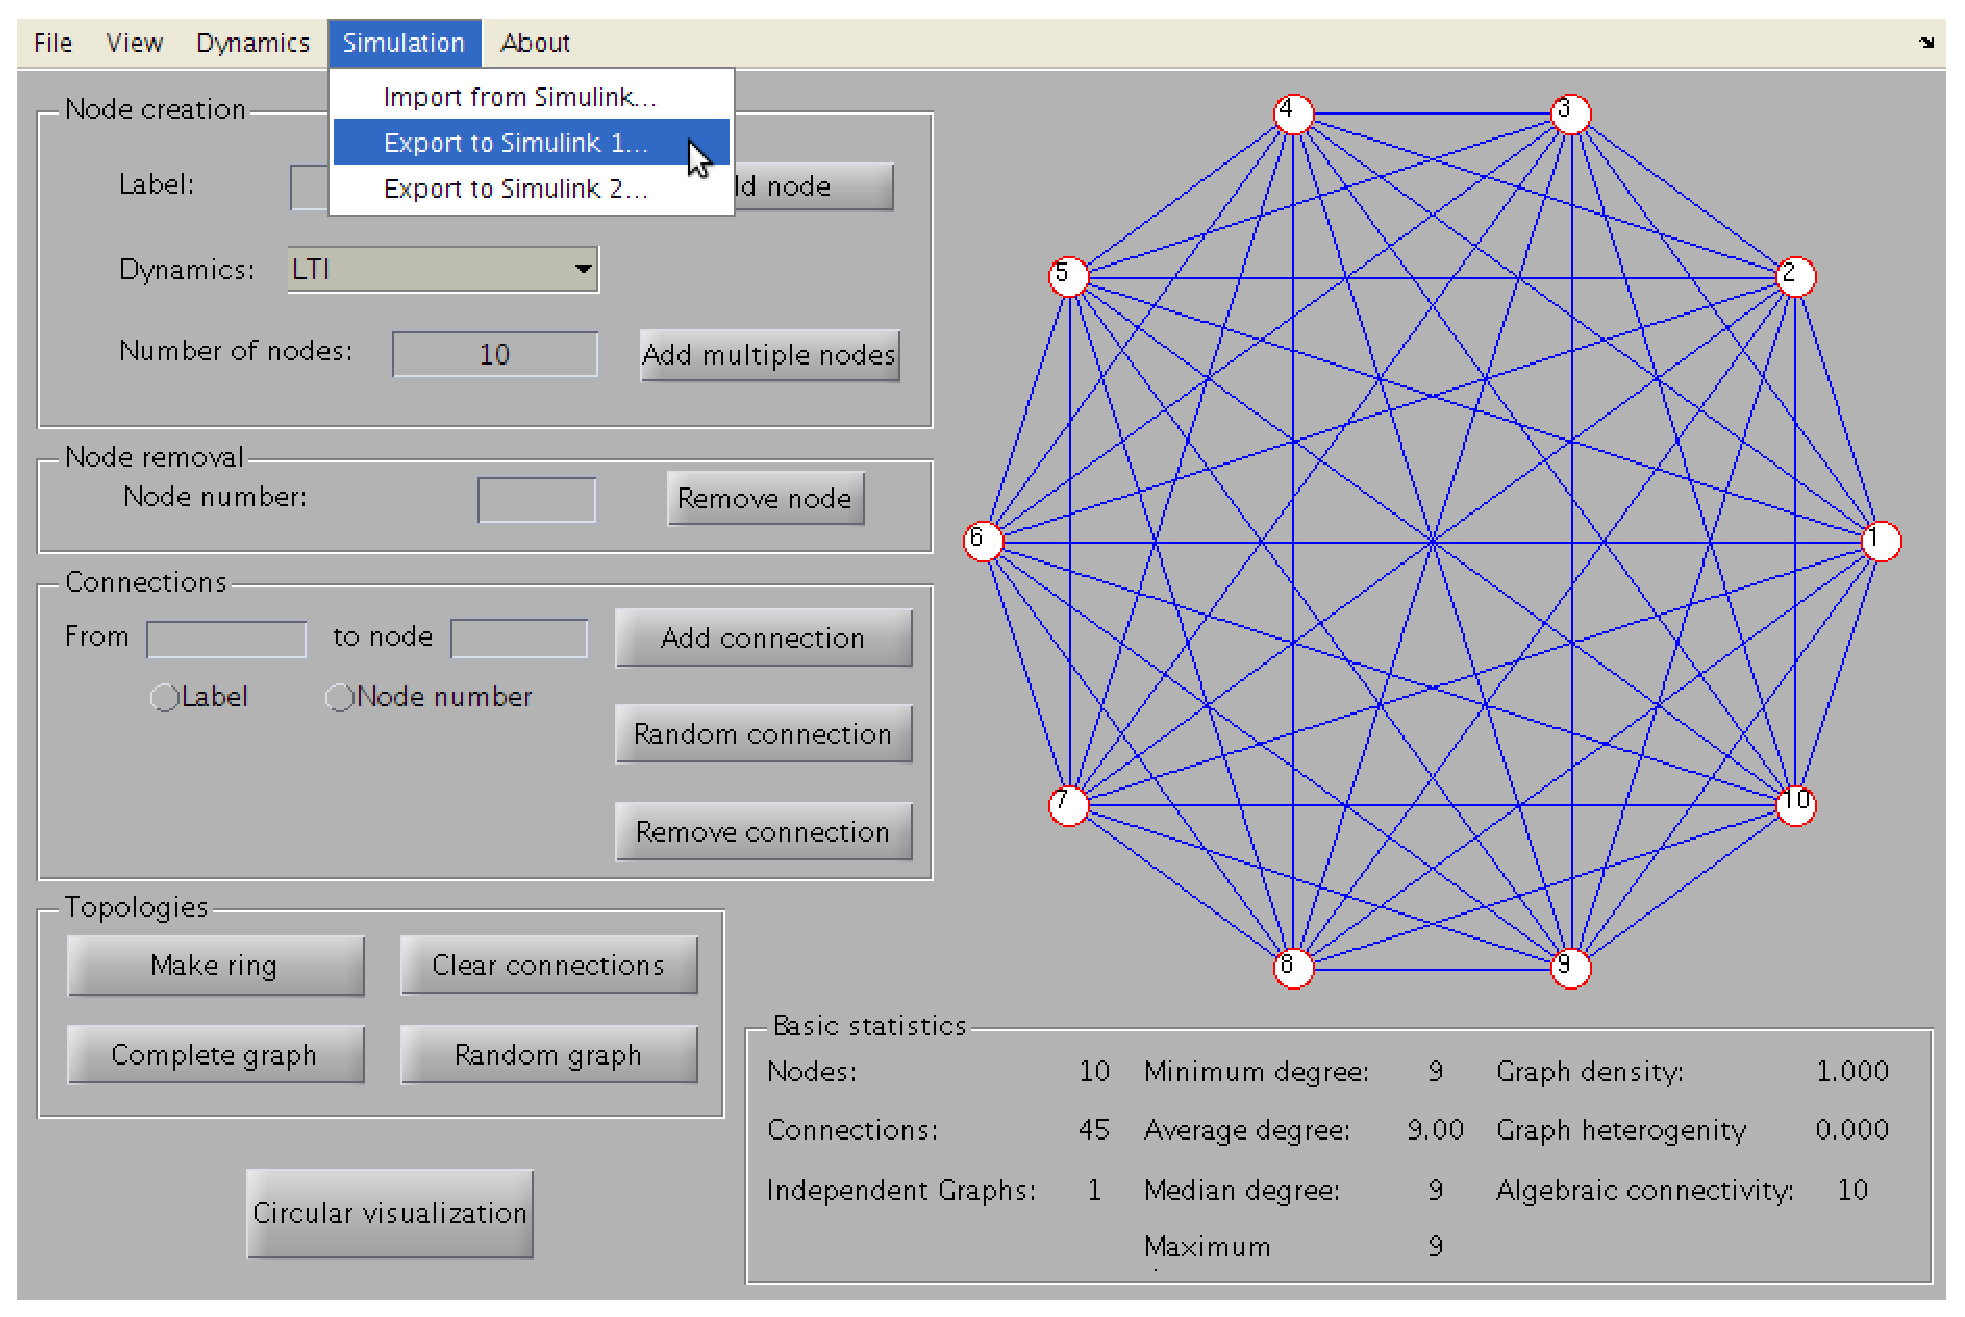
\includegraphics[width=0.7\textwidth]{pics/screenExport2.eps}
\caption[MTIDS export to Simulink]{MTIDS: export model to Simulink in the MTIDS format 1. Example is a complete graph with 10 LTI nodes.  }
\label{exportFig}
\end{figure}

The MTIDS GUI then calls the function exportSimulink.m, which builds a Simulink model with the following information:
model name, list of nodes' dynamics templates, list of templates that are available in mtids, adjacency matrix, position of the nodes and nodes' names. 
The result is a Simulink model in the MTIDS format. \\

To adjust the size of the model to the Simulink window size: \textbf{View $\rightarrow$ Fit System To View}\\
% 

\begin{figure}[htb]
\centering
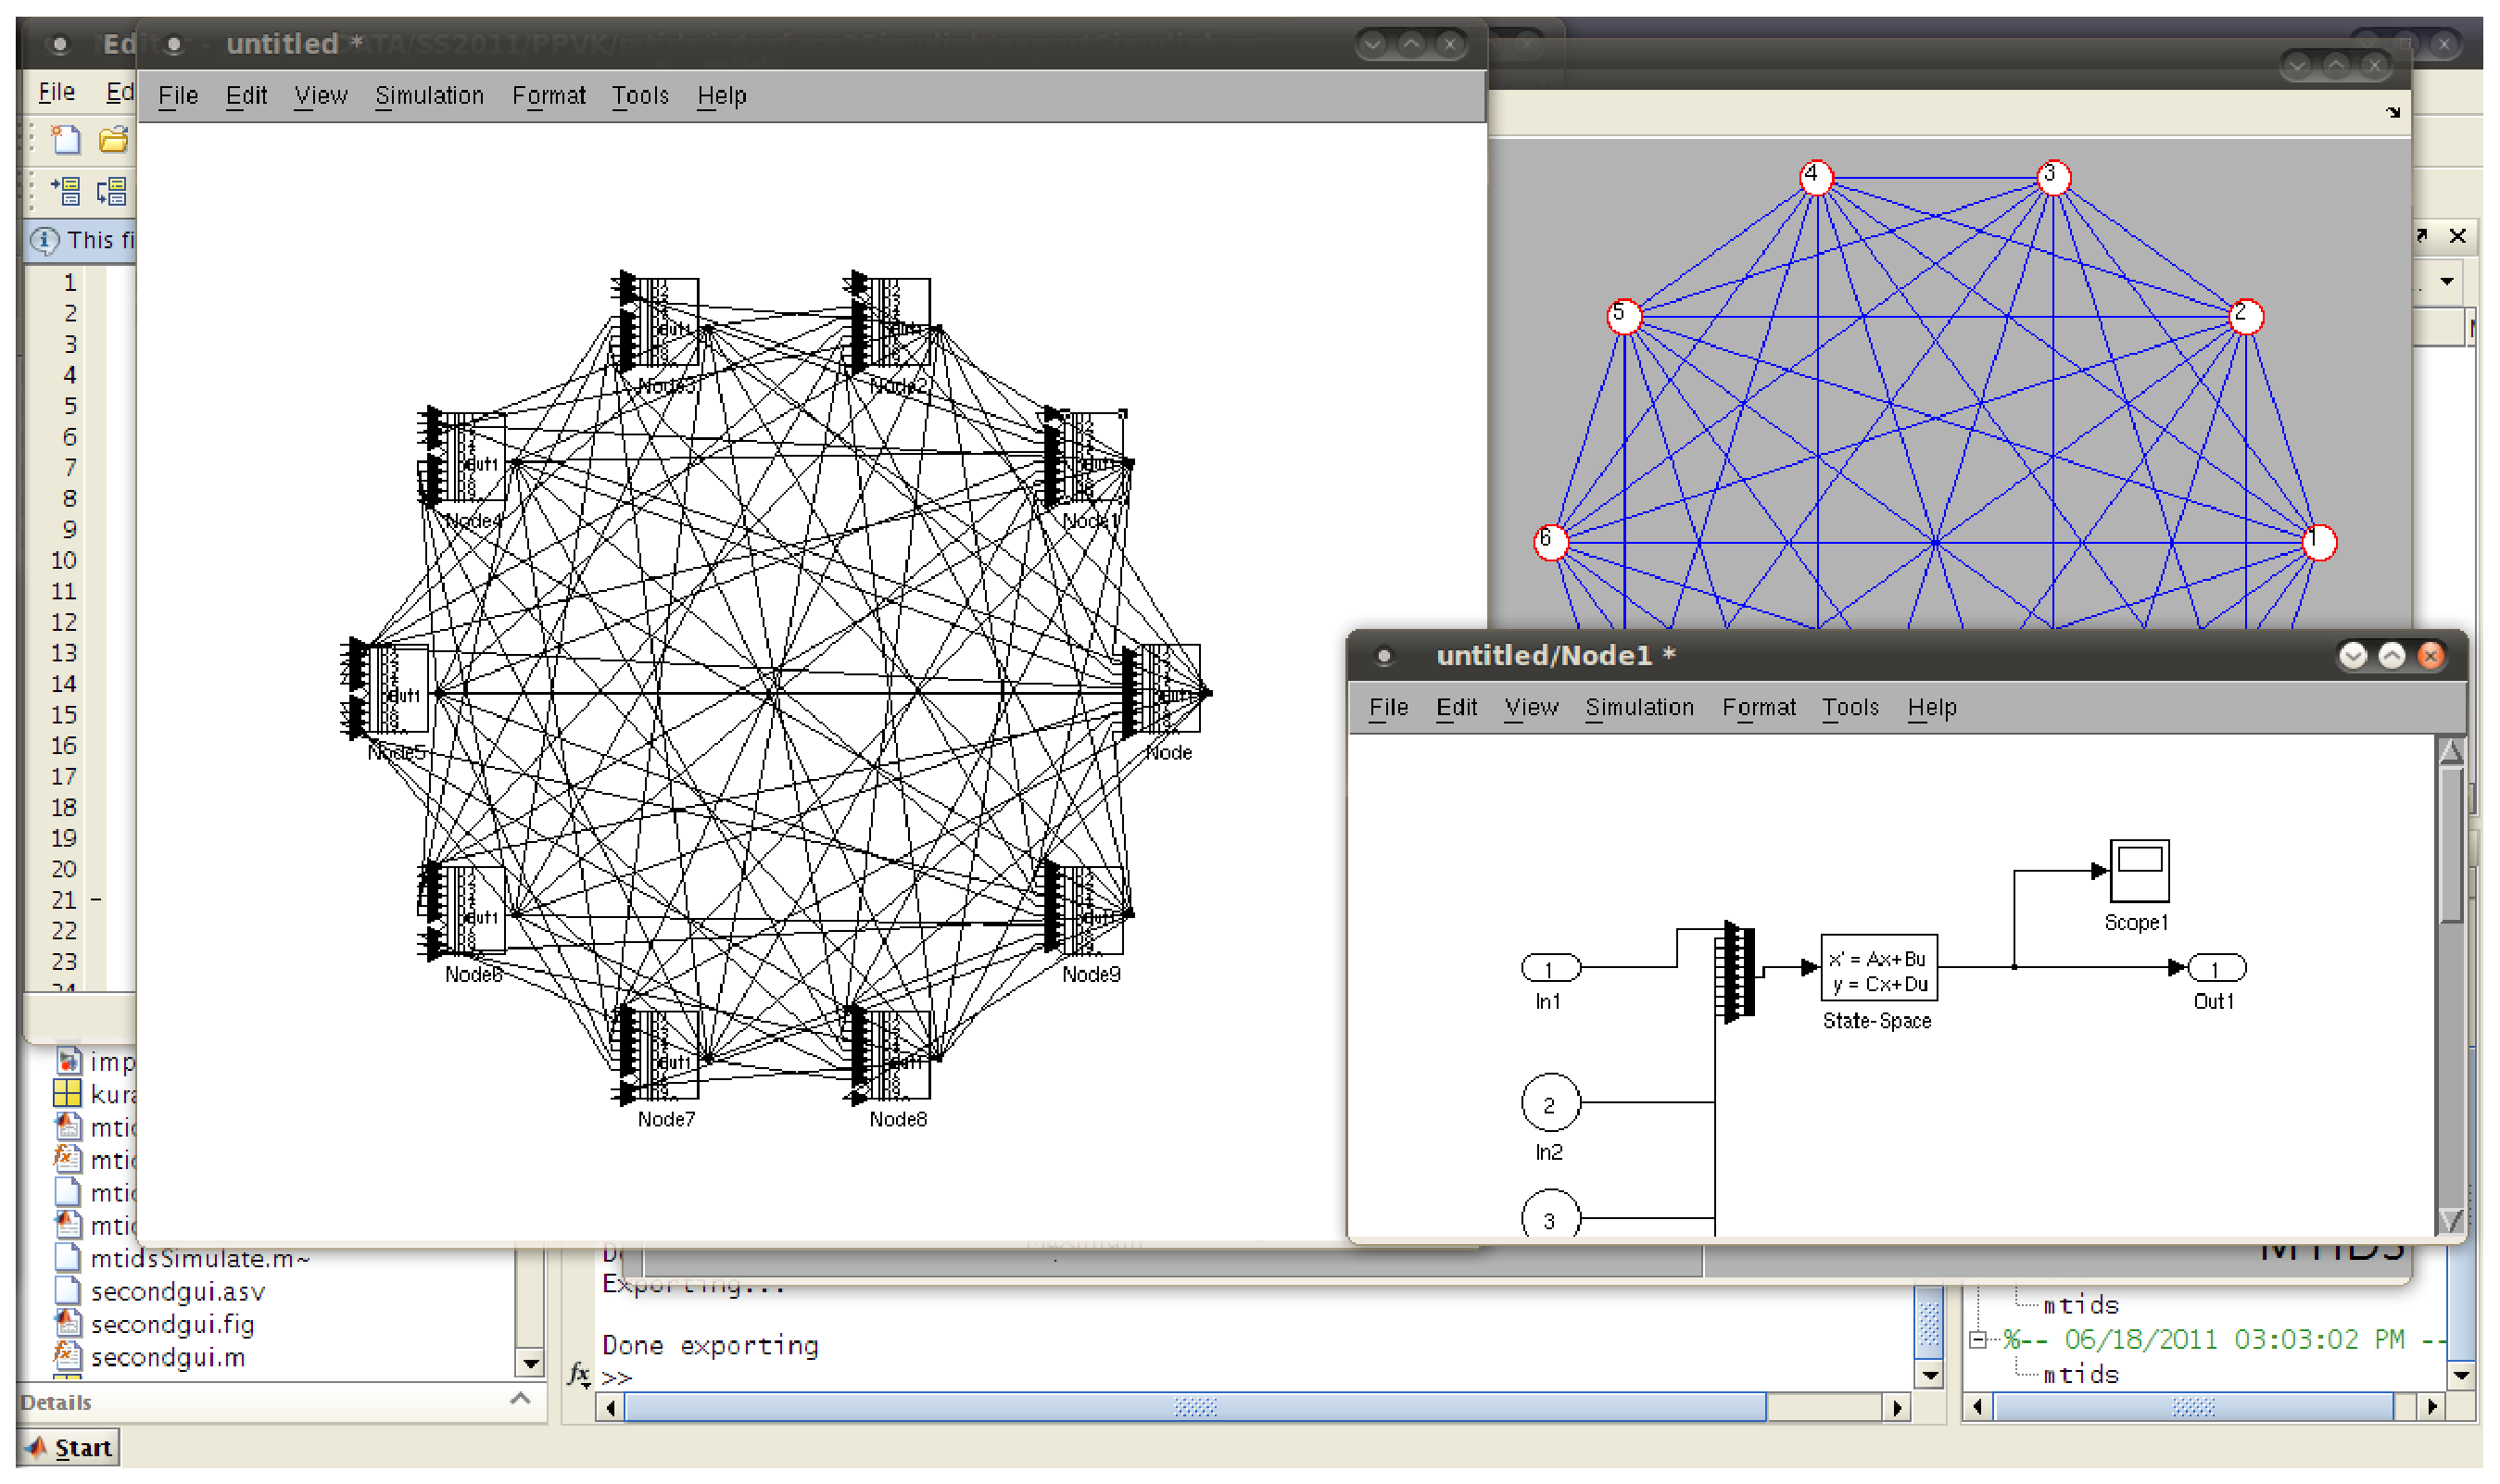
\includegraphics[width=0.7\textwidth]{pics/screenExportResult.eps}
\caption[MTIDS exported Simulink model]{Interconnected system Simulink Model. Example is a complete graph with 10 LTI nodes. }
\label{exportFig}
\end{figure}

In Figure \ref{exportFig}, the nodes are ordered in a circle, the topology of the system defined in MTIDS remains. The circle arrangement is a 
design decision, made, in order to allow a better access to the nodes. Each one of the nodes is a subsystem block. The dynamic of the nodes is defined inside
the subsystem block. Moreover, depending on the MTIDS export concept choosen, the number of inputs of a node will be different, compare with a zoom 
of the first node for our example in Figure \ref{nodeFig}. \\
 
\begin{figure}[htb]
\centering
\mbox{\subfigure[Node for concept 1]{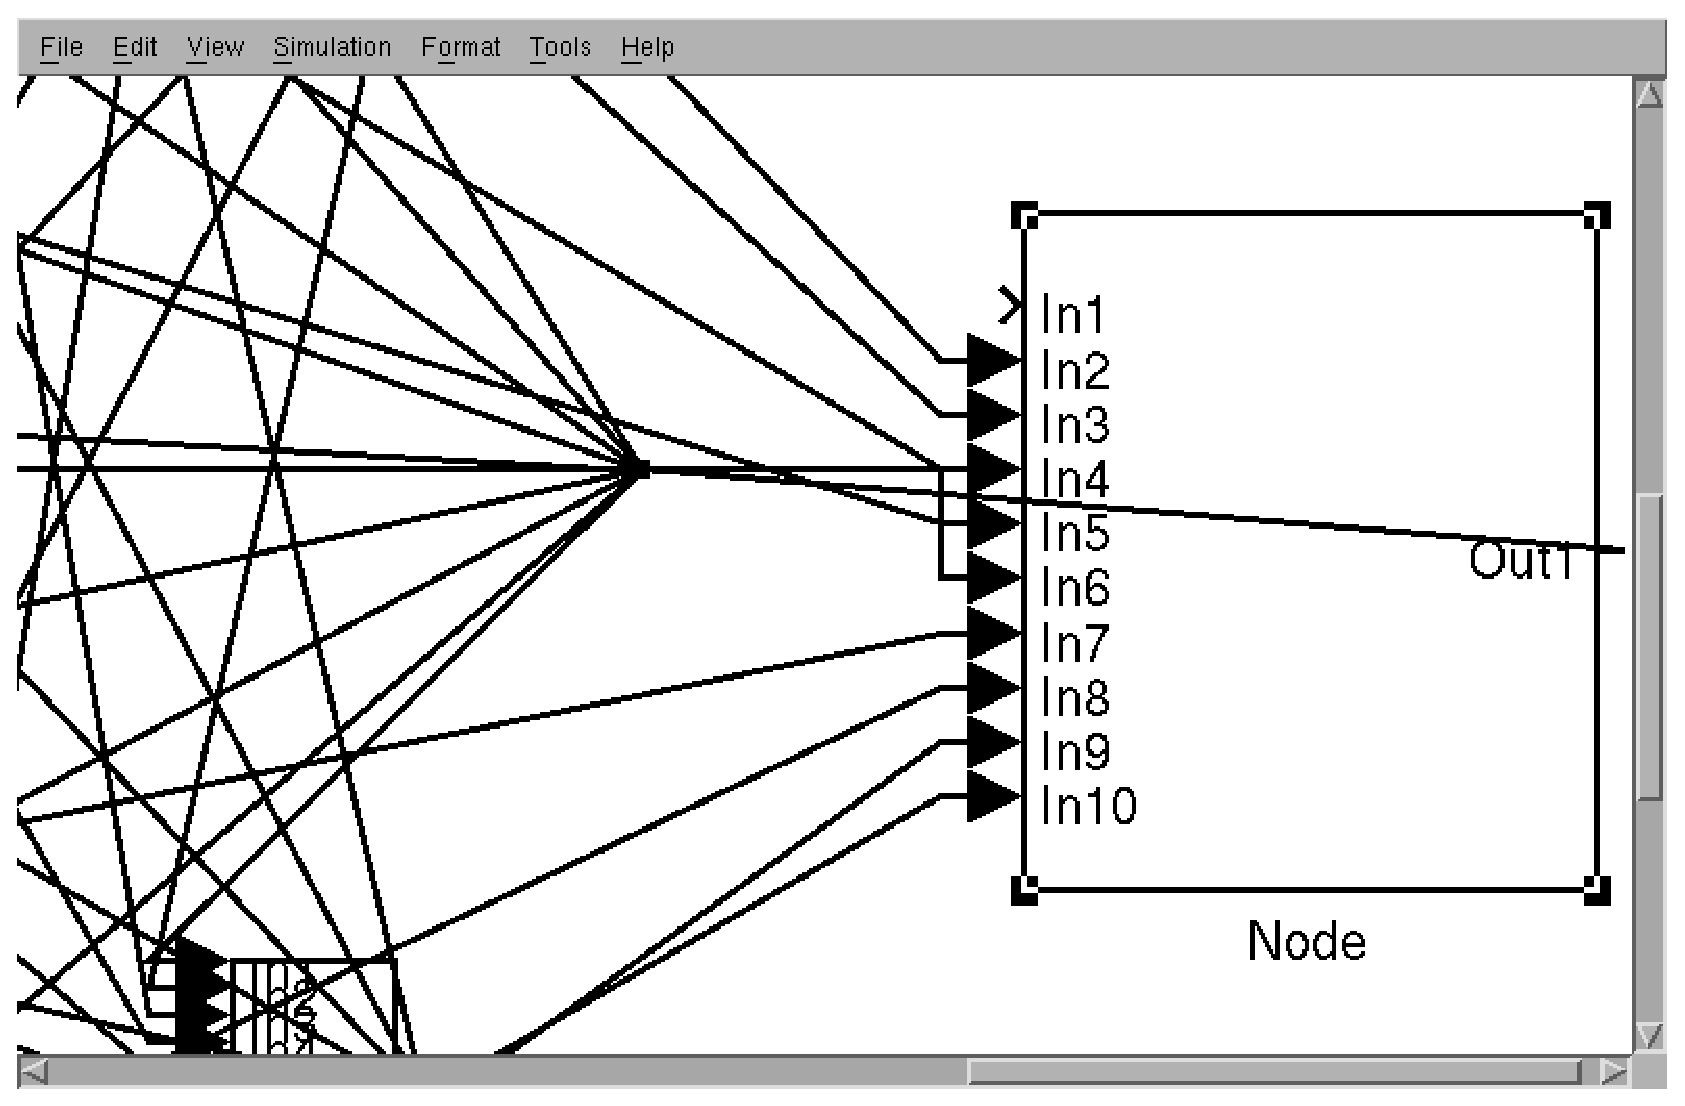
\includegraphics[width=.5 \textwidth]{pics/screenNode.eps} }\quad
\subfigure[Node for concept 2]{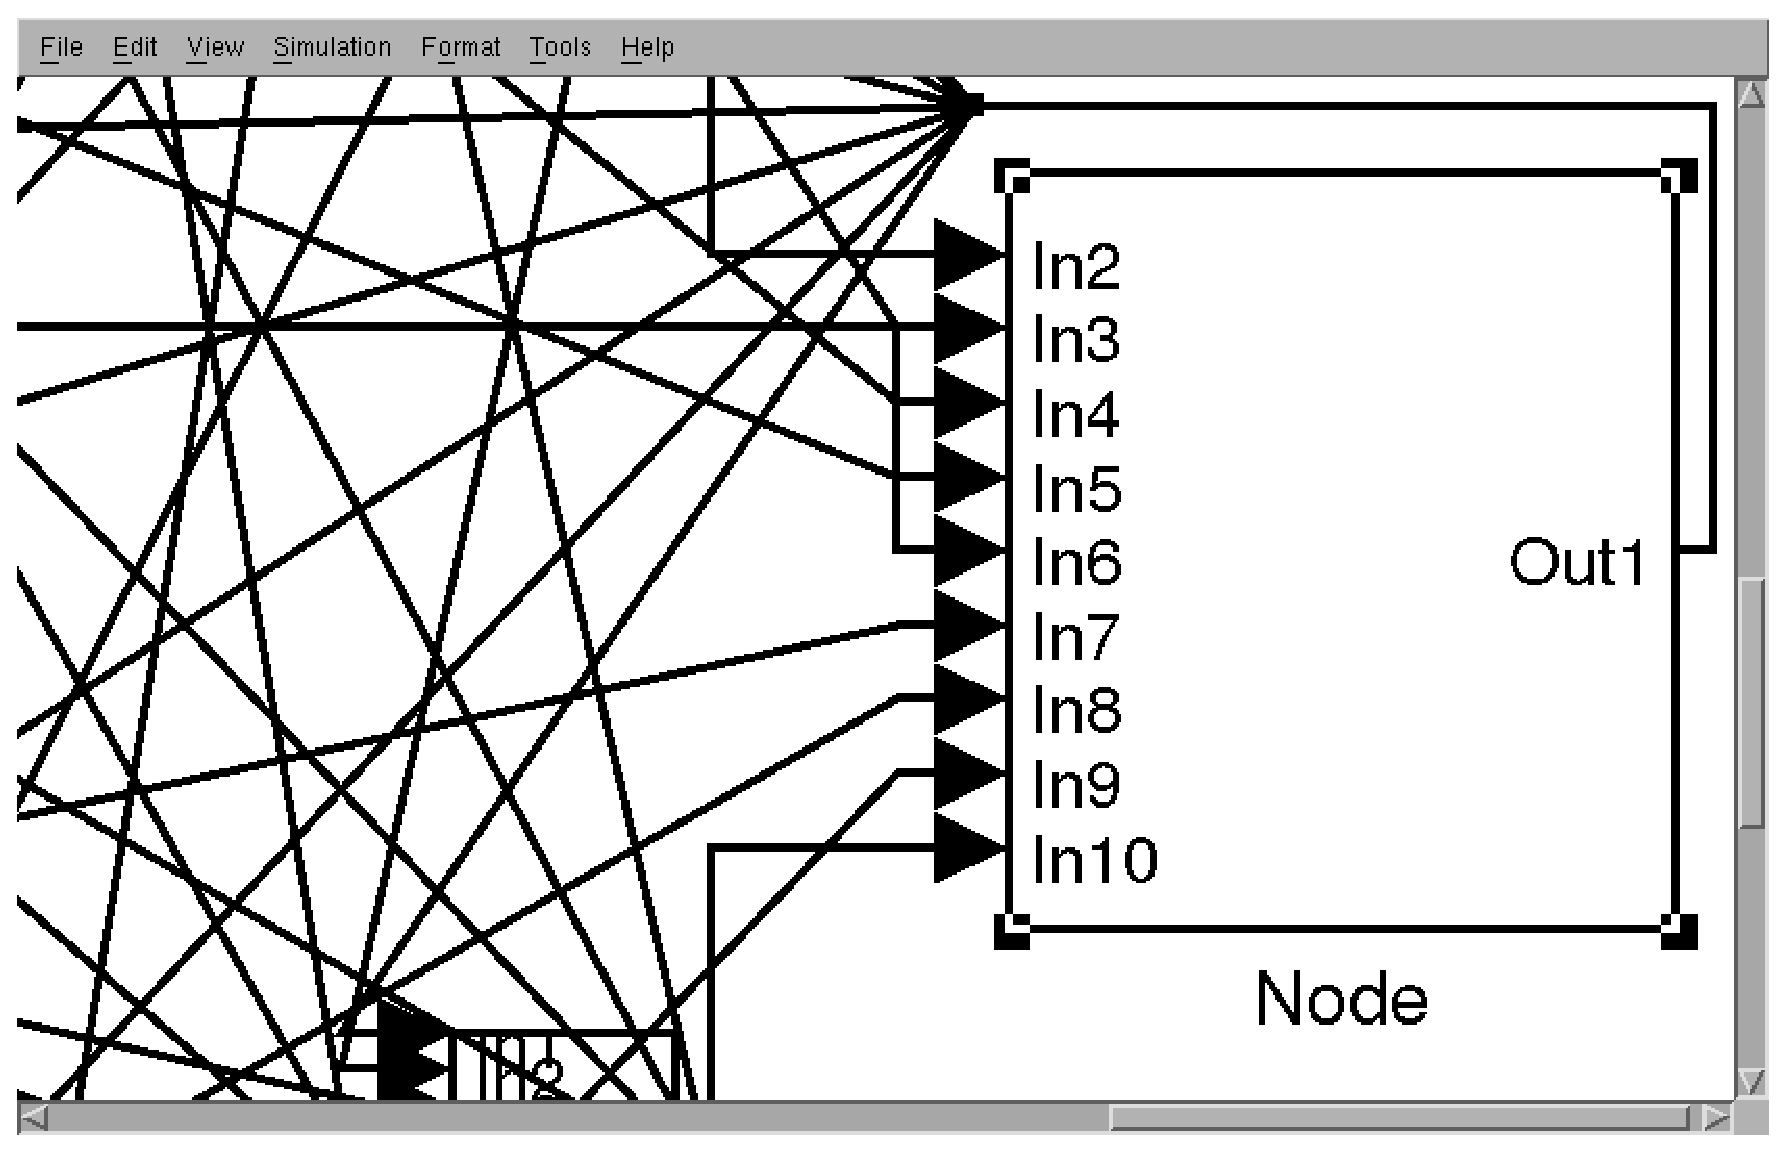
\includegraphics[width=.5\textwidth]{pics/screenConcept2.eps}  }}
\caption[MTIDS node in Simulink]{Node inputs and output: (a) Each node has an in-port for every node in the model and a single out-port. 
(b) Each node has an in-port for nodes connected to it and a single out-port. Example is the first node of a complete graph with 10 LTI nodes. }
\label{nodeFig}
\end{figure}

Notice that for concept 1 the port corresponding to the node's number
should always be free, e.g. the first node has an unconnected in-port 1, the second node an unconnected in-port 2, etc. For concept 2 all in-port are always connected. 
In case that a loop of a node with itself is required, we recommend doing this inside the subsystem/node. 
Another important aspect to point out is that when simulating the system, Simulink will issue a warning for unconnected in-ports and set their input to the subsystem to 0, this means 
that an \textbf{unconnected port enters the subsystem (local dynamics of the node) with a value of zero} during simulations. This can be exploited to 
make the parametrization of the nodes' dynamics easier. 

\section{Nodes' Dynamics}

As mentioned in the past section \ref{exportToSimulink} each node defined in MTIDS is exported to Simulink as a subsystem. The exportSimulink.m function 
uses predefined dynamic templates, which are modified according to the, in MTIDS, defined topology. Next, we explain how to define your own templates and
show how to use 2 preloaded templates: the LTI template and the kuramoto template. This templates can be found in the \textbf{/templates} directory. 


\subsection{Build your own Template} \label{nodeTemplate}
The real power of MTIDS depends on your ability to build templates. 
\\
\begin{figure}[htb]
\centering
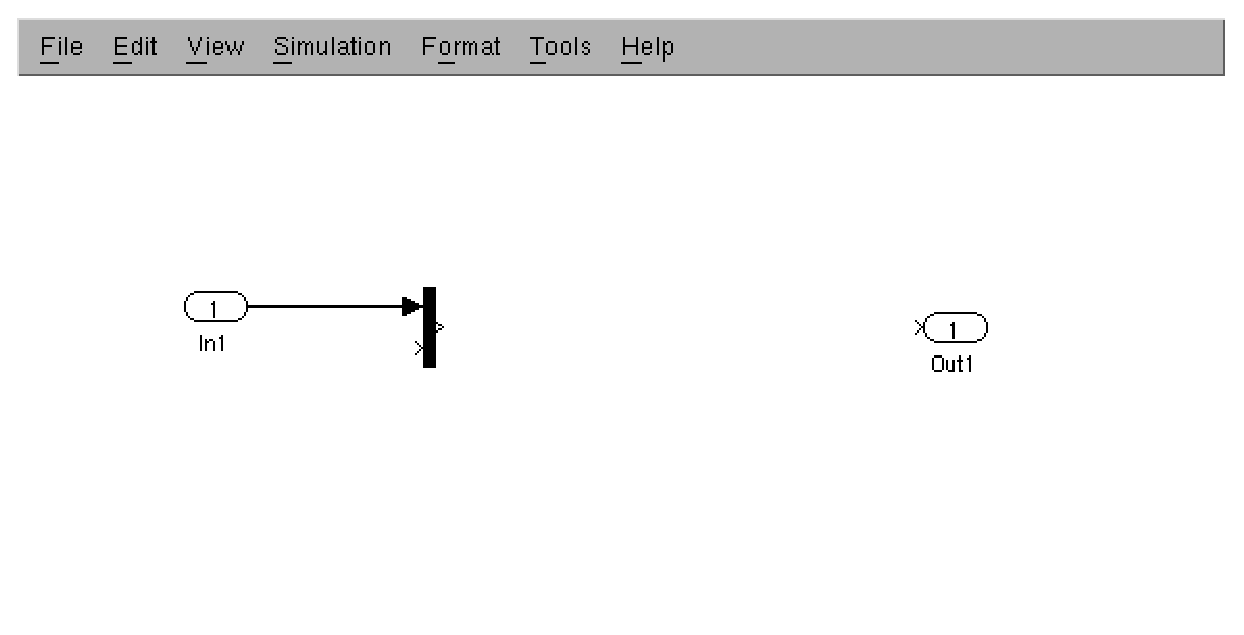
\includegraphics[width=0.6\textwidth]{pics/screenBuildTemplate.eps}
\caption[MTIDS node's scratch Template]{Scratch template for node's dynamics (\textbf{interfaceTemplate.mdl}). }
\label{templateFig}
\end{figure}

In Figure \ref{templateFig} we can see the components that each template should have: an in-port connected to a mux and an out-port.
Between the mux and the out-port you can design your own custom dynamics. The input to the system comes from the mux block as vector, which is composed by the values
entering the node/subsystem. The output of your system should also be aggregated to a vector and routed to the out-port. The separation of the different inputs and outputs 
is left to the system's designer. With a well thought architecture complex systems are very easy to achieve, please refer to the LTI and kuramoto template examples.  
\\

The dynamic of a node can be as simple as a junction that only reroutes the incoming signals or more complicated to include controllers and systems inside of it. It is this feature that allows
the implementation of clusters or layered systems, see subsection \ref{layering}. 


\subsection{The LTI template}

The LTI template is an example that defines a linear time invariant dynamic for nodes. The mathematical model 
of a simple interconnected LTI system as explained in \cite{LargeScaleSystems} can be written as:
\begin{eqnarray}
\left( \begin{array}{c}
\dot{x_1} \\  
\vdots \\
\dot{x_N}
\end{array} \right)=
\left( \begin{array}{ccc}
A_{11} & \cdots & A_{1N} \\  
\vdots & \ddots & \vdots\\
A_{N1} & \cdots &A_{NN}
\end{array} \right) 
\left( \begin{array}{c}
x_1 \\  
\vdots \\
x_N
\end{array} \right)+
\left( \begin{array}{c c c}
B_{1} & \cdots & B_{N}  
\end{array} \right) 
\left( \begin{array}{c}
u_1 \\  
\vdots \\
u_N
\end{array} \right)       
\end{eqnarray}
or
\begin{equation}
 \dot{x}=Ax+Bu
\end{equation}
The local view of a single subsystem/node (here for the first node) is:
\begin{eqnarray}
  \dot{x_1}= 
\left( \begin{array}{c c c c c c c}
A_{11} & A_{12} & \cdots & A_{1N} & B_{1} & \cdots & B_{N}  
\end{array} \right) 
\left( \begin{array}{c}
x_1 \\ 
x_2 \\ 
\vdots \\
x_N\\
u_1 \\  
\vdots \\
u_N
\end{array} \right)    
\end{eqnarray}
this can be reformulated as
\begin{eqnarray} \label{LTIFor}
 \dot{x_1}= A_{11}x_1 +  
\left( \begin{array}{c c c c c c c}
A_{11} & A_{12} & \cdots & A_{1N} & B_{1} & \cdots & B_{N}  
\end{array} \right) 
\left( \begin{array}{c}
0 \\ 
x_2 \\ 
\vdots \\
x_N\\
u_1 \\  
\vdots \\
u_N
\end{array} \right) 
\end{eqnarray}





In order to keep things simple, we define the local output of each node as
\begin{eqnarray}
 y_i=  x_i,\ \mbox{for}\ i=1,\ldots,N. 
\end{eqnarray}

To implement this dynamic as a template we make use of the State-Space block.

\begin{figure}[htb]
\centering
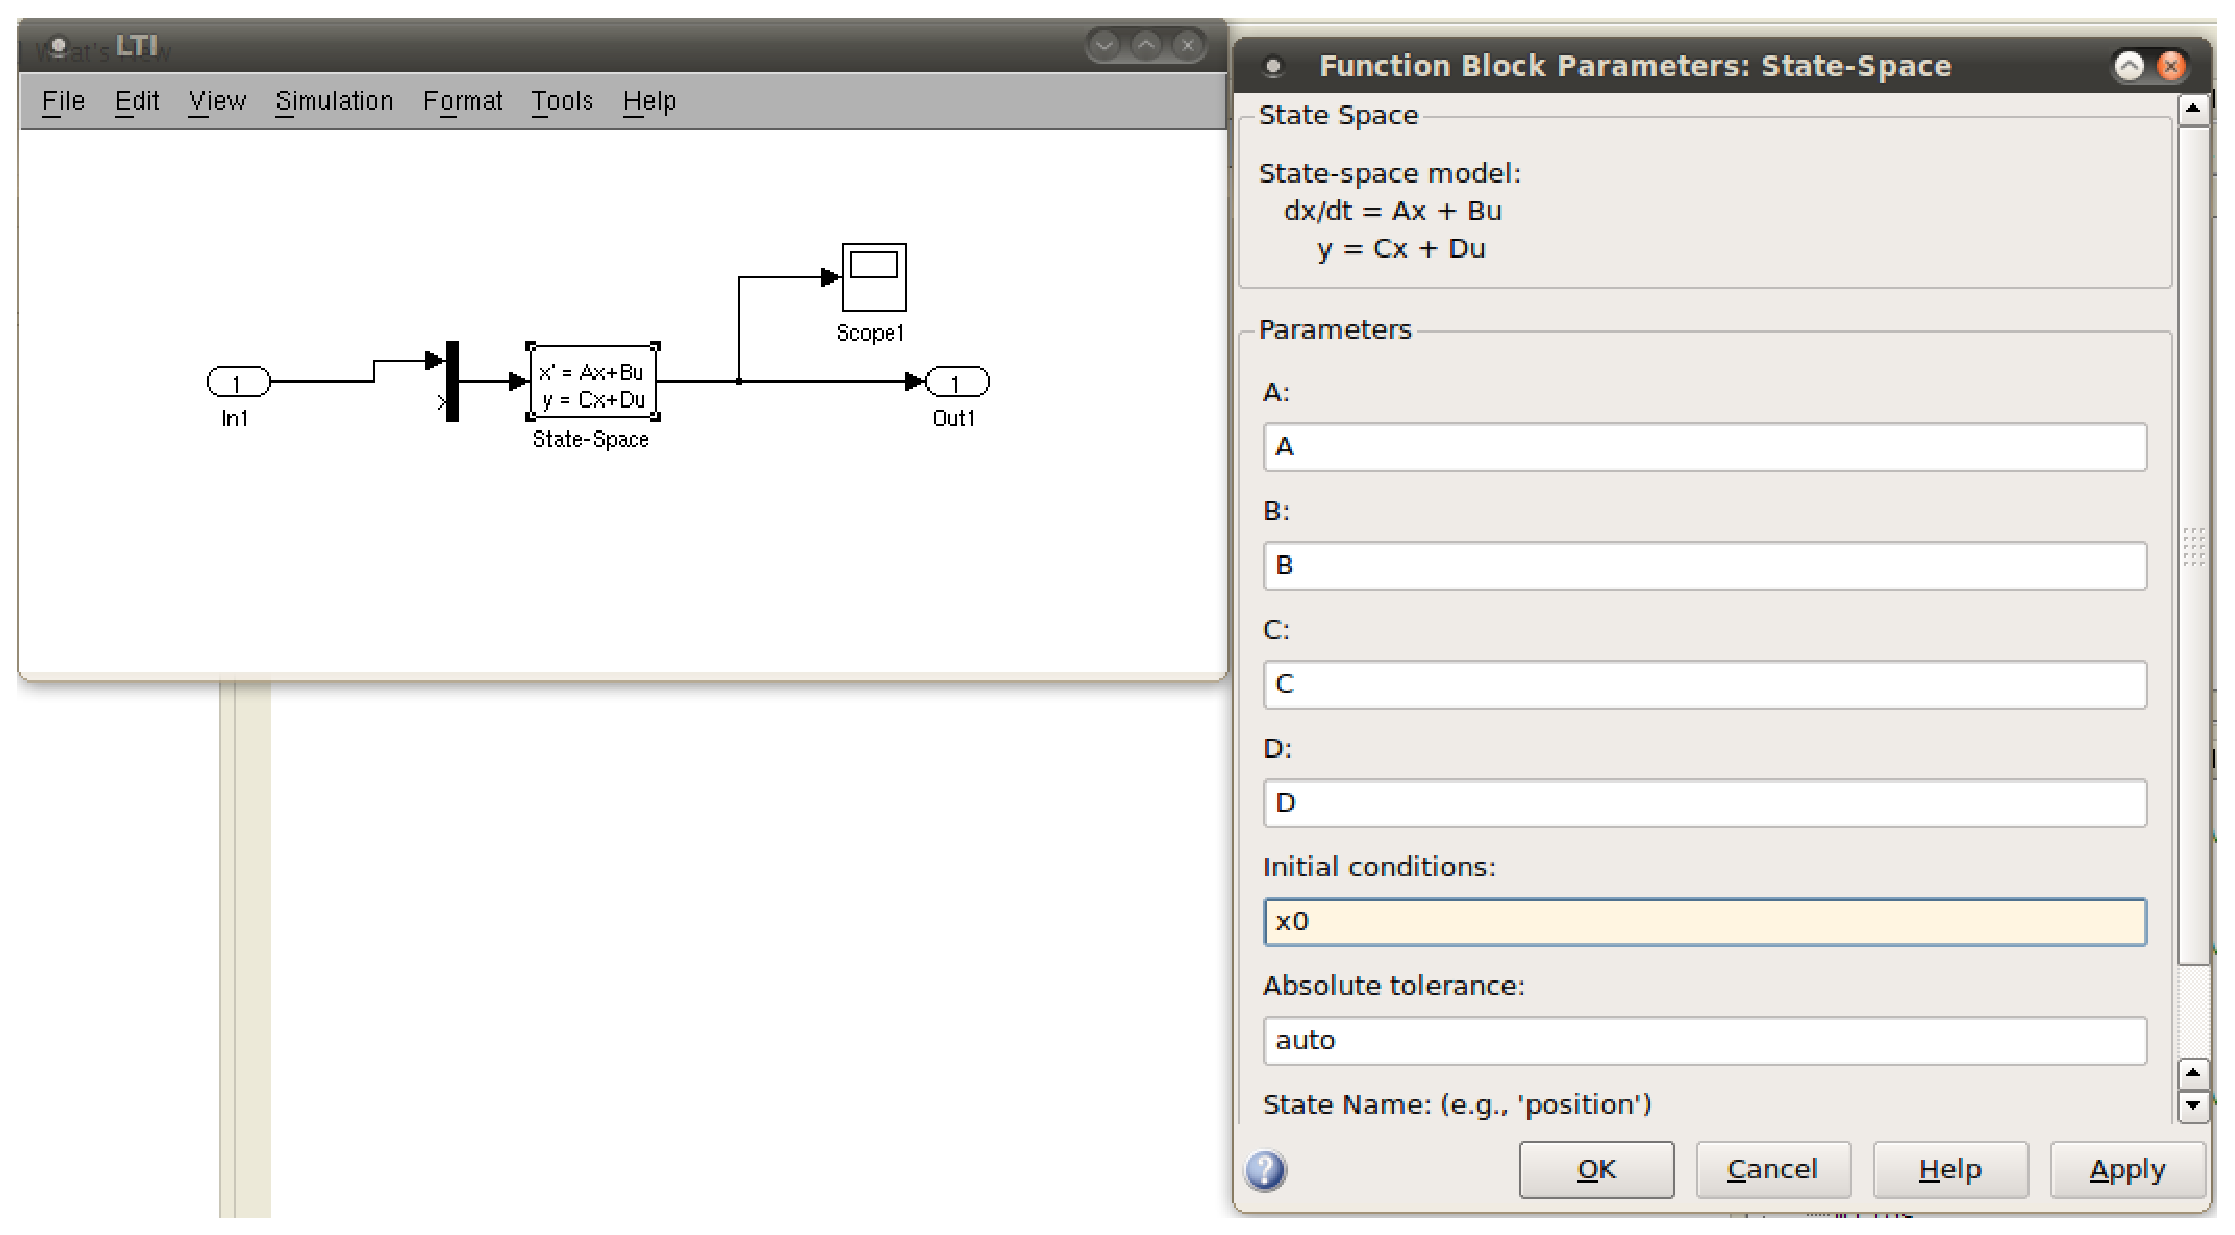
\includegraphics[width=0.8\textwidth]{pics/screenLTI.eps}
\caption[MTIDS LTI Template]{LTI template,  \textbf{/templates/LTI.mdl}}
\label{templateLTIFig}
\end{figure}
 
The LTI template shown in Figure \ref{templateLTIFig} can be used in MTIDS to create interconnected LTI systems with different topologies. One way to avoid 
the work of parameterizing the A,B,C and D matrix of every node separately, is to define the same matrix for all subsystems. Using formula 
(\ref{LTIFor}) and exporting with \textbf{concept 1} we can define an A, B, C, and D matrix for every node. An example can be
\begin{eqnarray}
 A&=& 1\nonumber\\
B&=&[-1 \cdots -1]^{1\times N}\nonumber\\
C&=& 1\nonumber\\
D&=& [0 \cdots 0] ^{1\times N}\nonumber
\end{eqnarray}

As the in-port corresponding to the node itself is automatically set to zero by Simulink during the simulation, we can define the same matrices for all 
nodes without getting any errors.
\\

For more complicated LTI models we recomend creating many different LTI templates.

\subsection{The Kuramoto Template}
The kuramoto template is an example of a non-linear dynamic for a node. This kuramoto model is used to model the behavior of coupled oscillators. One of the interesting behaviors
that may occur in this type of systems is synchronization. The mathematical equation of $N$ coupled oscillators is written for each oscillator $i$ as
\begin{equation}\label{kuramotoFor}
 \dot{\theta_i} = \omega_i + \frac{K}{N} \sum_{j=1}^N \sin(\theta_j-\theta_i). 
\end{equation}



\begin{figure}[htb]
\centering
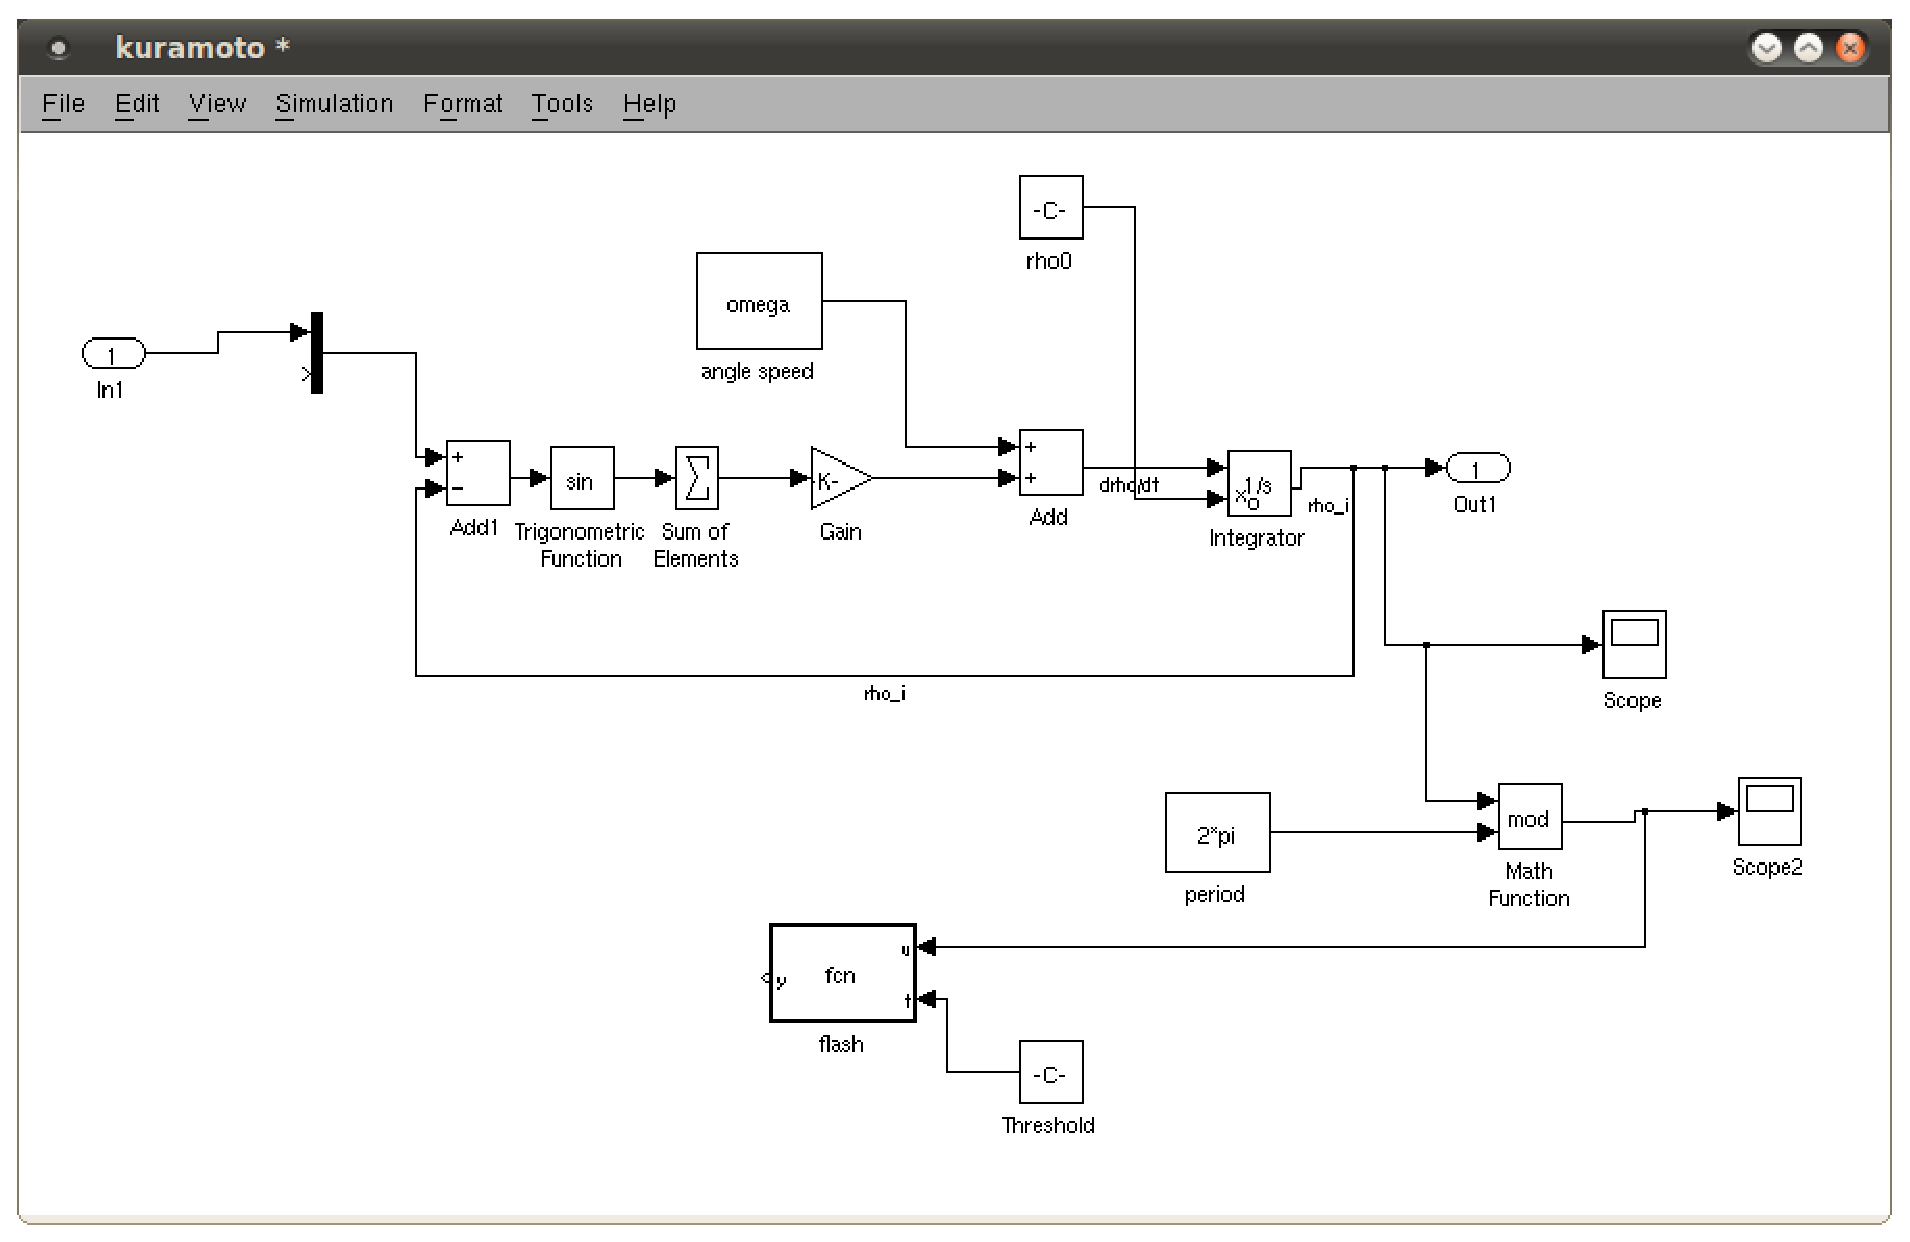
\includegraphics[width=0.6\textwidth]{pics/screenKuramoto.eps}
\caption[MTIDS Kuramoto Template]{Kuramoto template for fireflies synchronization, \textbf{/templates/kuramoto.mdl}}
\label{templateKuramotoFig}
\end{figure}
 
In Figure \ref{templateKuramotoFig} we see  the MTIDS's kuramoto template after formula (\ref{kuramotoFor}). The goal was to model fireflies synchronization, thus
the model has an embedded function that changes the color of the parent block for a defined threshold, this mimics the flashing of a firefly.
With the right parameters one can build a synchronizing firefly colony using MTIDS. Remember that the kuramoto.mdl template needs to be added in MTIDS:
Dynamics $\rightarrow$ Add mdl template. You also need to set up the right parameters for synchronization, an example can be seen in Figure \ref{syncFig}.
In order to see the blinking in the correct time scale, you need to set up the simulation with a fixed step size in Simulink, more on this in section 
\ref{workinginsimulink}. An \textbf{example} can be found under \textbf{demos/firefliesTemplate.mdl} with the parameters \textbf{firefliesTemplate.mat}.

\begin{figure}[htb]
\centering
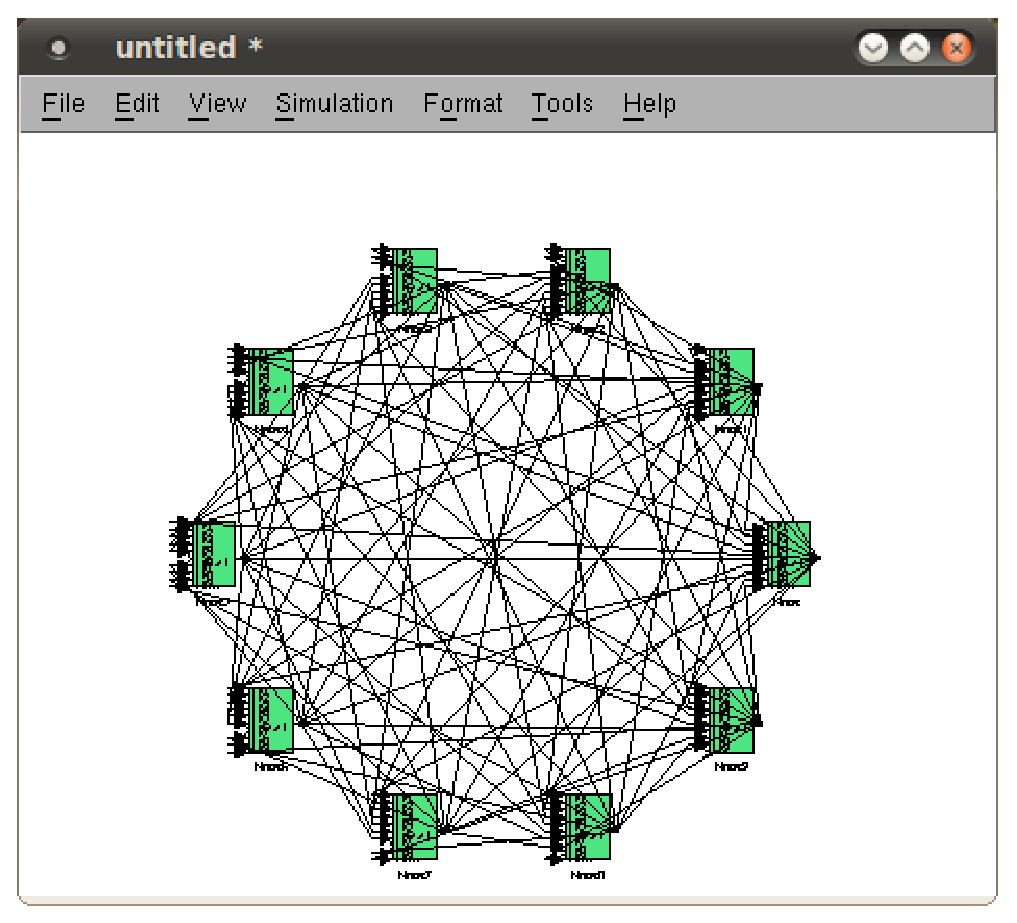
\includegraphics[width=0.4\textwidth]{pics/screenfireflies.eps}
\caption[MTIDS fireflies synchronization]{Simulation of 10 fireflies synchronizing, exported using concept 2. Parameters: K=0.1, N=10, $\omega=0.3$, $\theta_0=10$, var=5 (variation of starting point), threshold= $3/4*2\pi$}
\label{syncFig}
\end{figure}

\subsection{The Consensus Problem Templates}

The consensus or rendevous problem is a classic formulation where we see how a distributed hostless algorithm with simple
local interactions can achieve a well understood and studied global interaction.

A graph built in MTIDS using consensus nodes should be exported using the \textbf{Export to Simulink mode 2} 


\subsubsection{Follower node:}
The consensus follower template (/templates/consensus.mdl) contains a simple local dynamical model using standard Simulink blocks (see Figure \ref{templateConsensusFig}).
 This model is the realization of the local (decoupled) model is (as in \cite{NCS}):
\begin{equation}
\dot{x}_i = - \gamma \sum_{j=1}^{N_v(i)}(x_i - x_j)
\end{equation}
Every internal integrator state is initialized on random before the simulation.
\begin{figure}[htb]
\centering
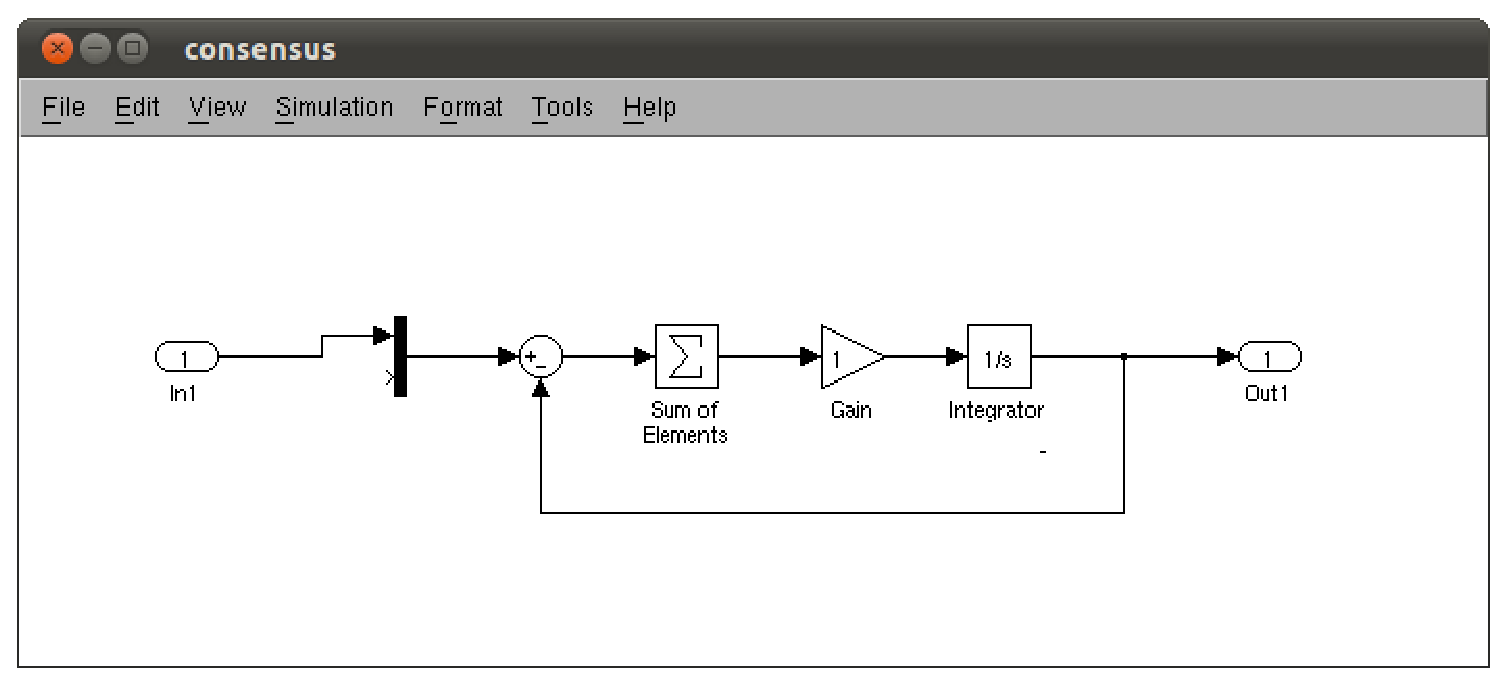
\includegraphics[width=0.6\textwidth]{pics/consensus_template.eps}
\caption[MTIDS Consensus Template]{Consensus template, \textbf{/templates/consensus.mdl}}
\label{templateConsensusFig}
\end{figure}
As an example we built in MTIDS a graph containing 6 consensus follower nodes as shown on Figure \ref{ConsensusGraphFig}.
The results of the simulation are shown on Figure \ref{ConsensusStatePlotFig}. It is easily recognizable that all nodes tend to a common state.

\begin{figure}[htb]
\centering
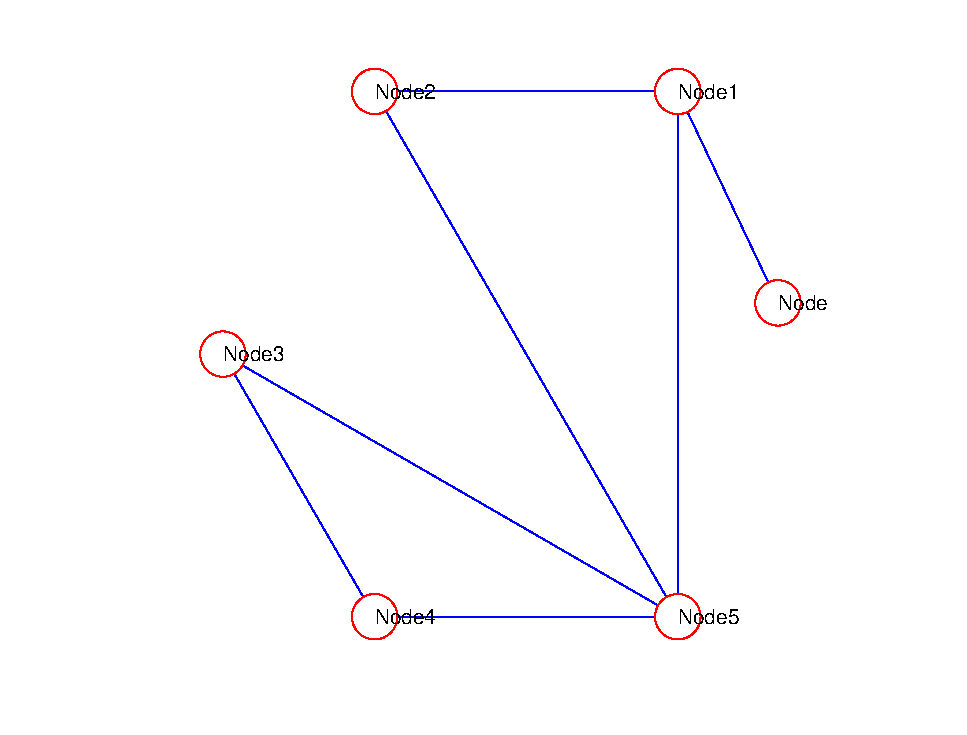
\includegraphics[width=0.6\textwidth]{pics/consensus_graph.eps}
\caption[Consensus Graph Example]{Consensus Graph Example}
\label{ConsensusGraphFig}
\end{figure}

\begin{figure}[htb]
\centering
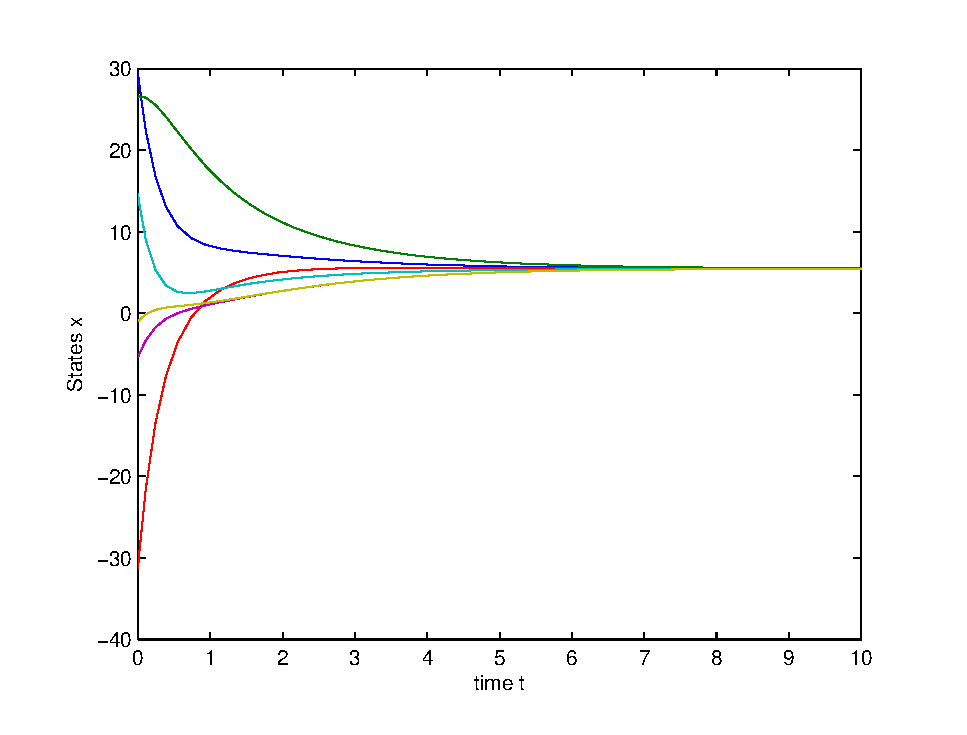
\includegraphics[width=0.6\textwidth]{pics/consensus_fig.eps}
\caption[Consensus State Plot]{Consensus State Plot}
\label{ConsensusStatePlotFig}
\end{figure}
\pagebreak

\subsubsection{Static Leader:}

A static leader node is a node which stays on a specific point in state-space.
It has following dynamics:

\begin{equation}
\dot{x}_i = 0
\end{equation}

\begin{equation}
  x_i(t) = x_0
\end{equation}

\begin{figure}[htb]
\centering
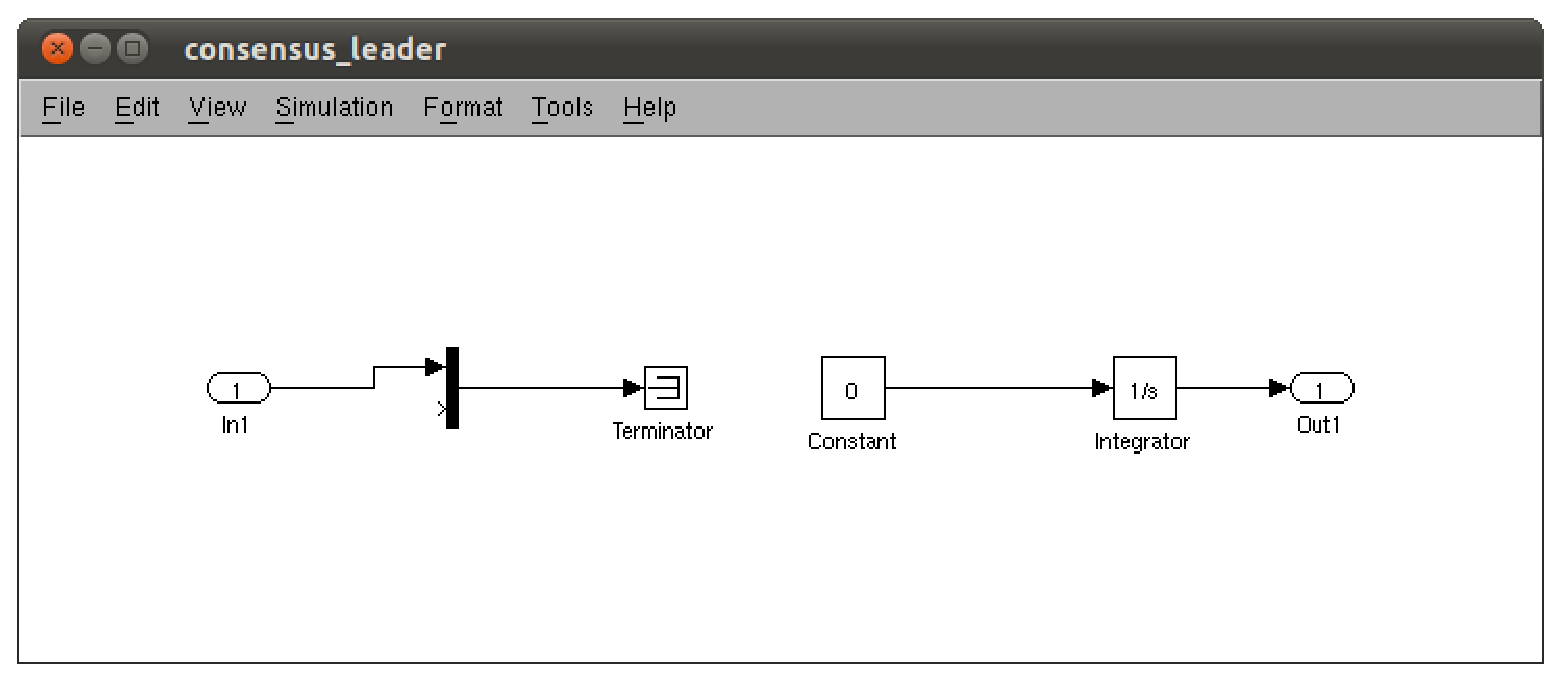
\includegraphics[width=0.6\textwidth]{pics/consensus_leader_template.eps}
\caption[MTIDS Consensus Leader Template]{Consensus leader template, \textbf{/templates/consensus leader.mdl}}
\label{templateConsensusLeaderFig}
\end{figure}

\subsubsection{linmod() Example with the Consensus Problem:}
Matlab function linmod() extracts a continuos linearized state-space model of a system around the operating point.
Every block inside the main system is linearized individually. The outputs of this function are the standard A,B,C,D matrices of an LTI-model.
Usage of linmod: \verb|[A,B,C,D] = linmod(sys)|.

We see that the result shown in Figure \ref{ConsensusLinmodFig} correspond to the negative of the Laplacian matrix of the graph shown in Figure \ref{ConsensusGraphFig}.
The output of linmod() can be used as a LTI-system which to be analysed using the Matlab Control Toolbox for stability, controller synthesis, etc. 
\begin{figure}[htb]
\centering
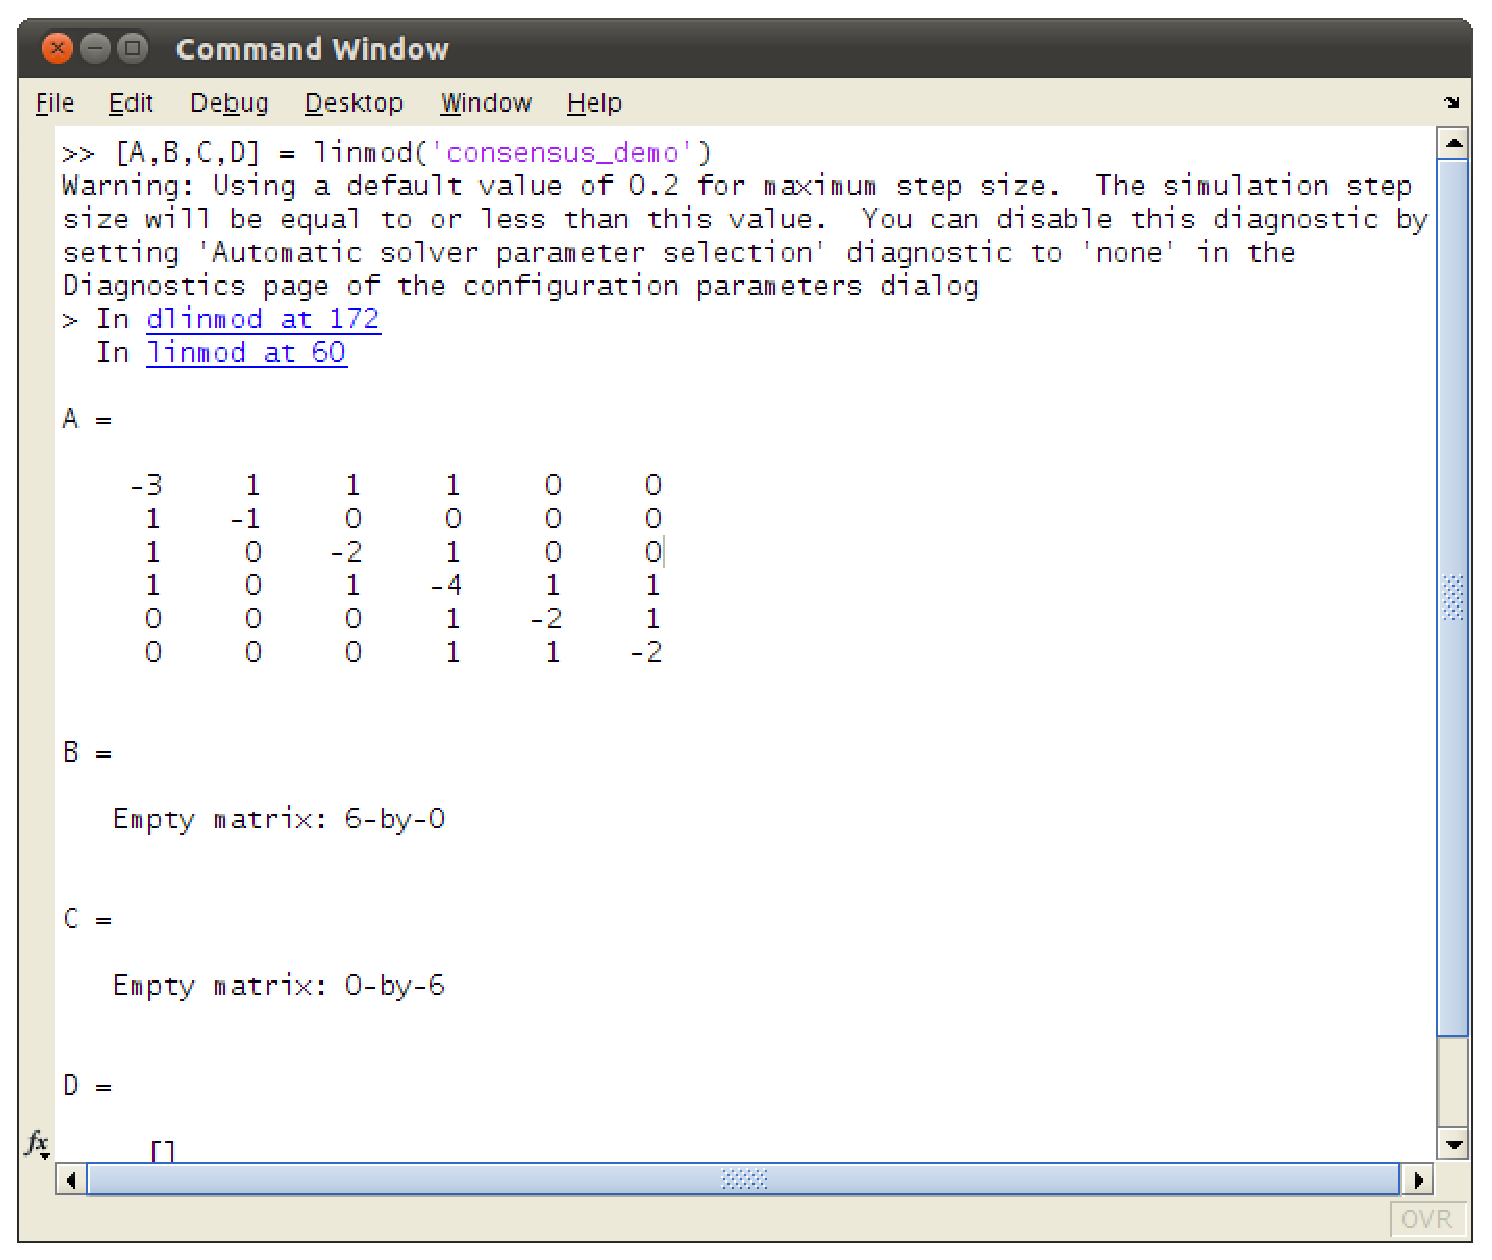
\includegraphics[width=\textwidth]{pics/Consensus_linmod.eps}
\caption[linmod() Example Output]{linmod() example output}
\label{ConsensusLinmodFig}
\end{figure}

\pagebreak
\section{Layering/Clustering Nodes} \label{layering}


The \textbf{key} to implement layering and clustering in MTIDS is the \textbf{interface node}. On clustered/layered interconnected systems there is always an interface
that regulates the data communication of one layer/cluster to other layers/clusters. The interface has access to all nodes in the current cluster/layer and 
on most cases does some information processing (compression, principal component extraction, etc). This processed information is used to interact with 
other clusters/layers. Inside the cluster/layer the interface node acts like a normal node.
\\

\subsection{Create a layer/cluster}

In oder to create a layer/cluster in MTIDS you need to export your system as a layer: \textbf{File $\rightarrow$ Export as a layer 1} for concept 1 or
\textbf{File $\rightarrow$ Export as a layer 2} for concept 2.\\

MTIDS will ask you to select a template for the interface node. You may select an interface node created by you or select the MTIDS provided
interface node : \textbf{layerInterface.mdl}.\\
The result is a Simulink model that differs from the one that MTIDS normally produces, as it includes an extra node, the interface node.
If we look more closely in Figure \ref{layerFig}, we notice that this model also fulfills the requirements needed to build a standard node template, see subsection \ref{nodeTemplate}.
By saving this model and using it as a node template in MTIDS we can build many of this interconnected systems, which interact with each other through their 
interface nodes, see Figure \ref{layersFig}. An \textbf{example} can be found under \textbf{demos/clusterDemo.mdl} with the parameters \textbf{clusterDemo.mat}.


\begin{figure}[htb]
\centering
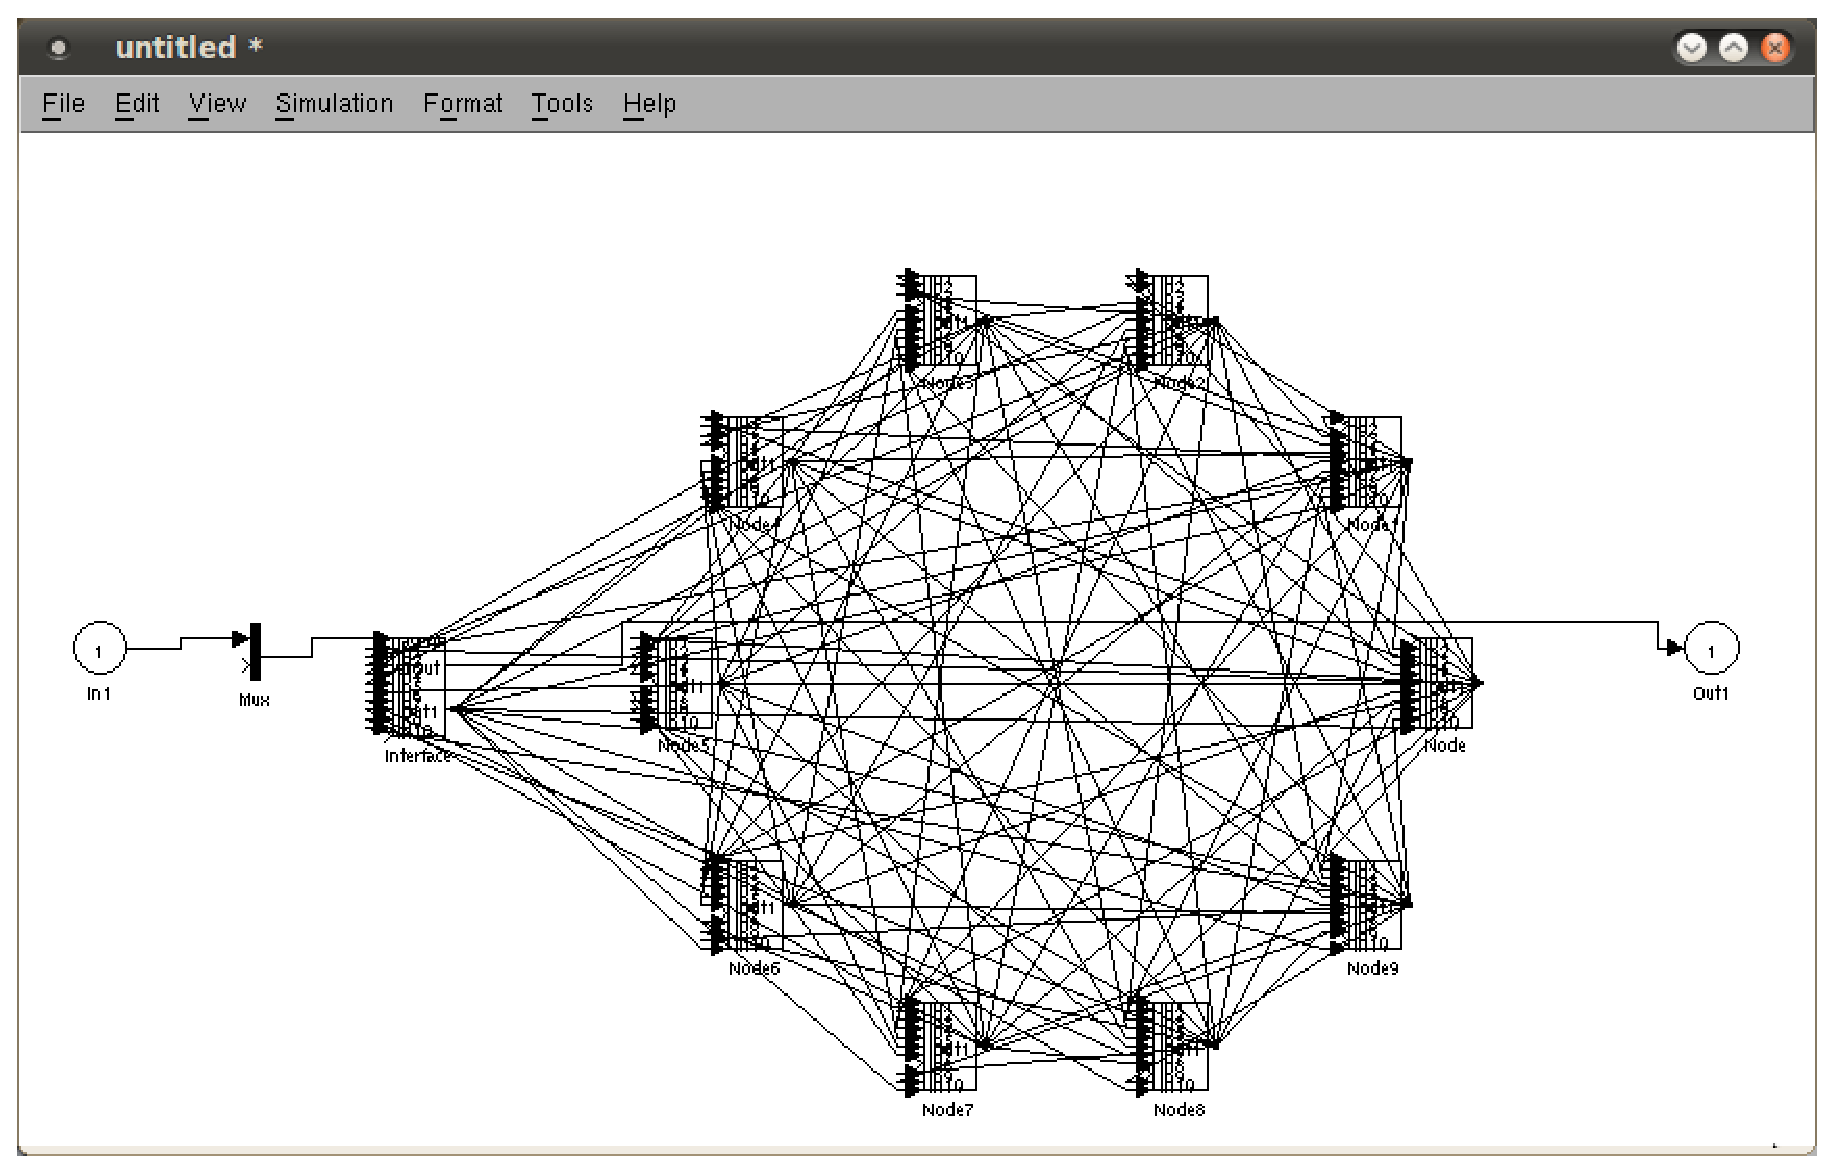
\includegraphics[width=0.5\textwidth]{pics/screenLayer.eps}
\caption[MTIDS export as layer resulting model]{Resulting layer/cluster when exporting in MTIDS as layer. Example is a complete graph with 10 LTI nodes, build using concept 1.}
\label{layerFig}
\end{figure}



\begin{figure}[htb]
\centering
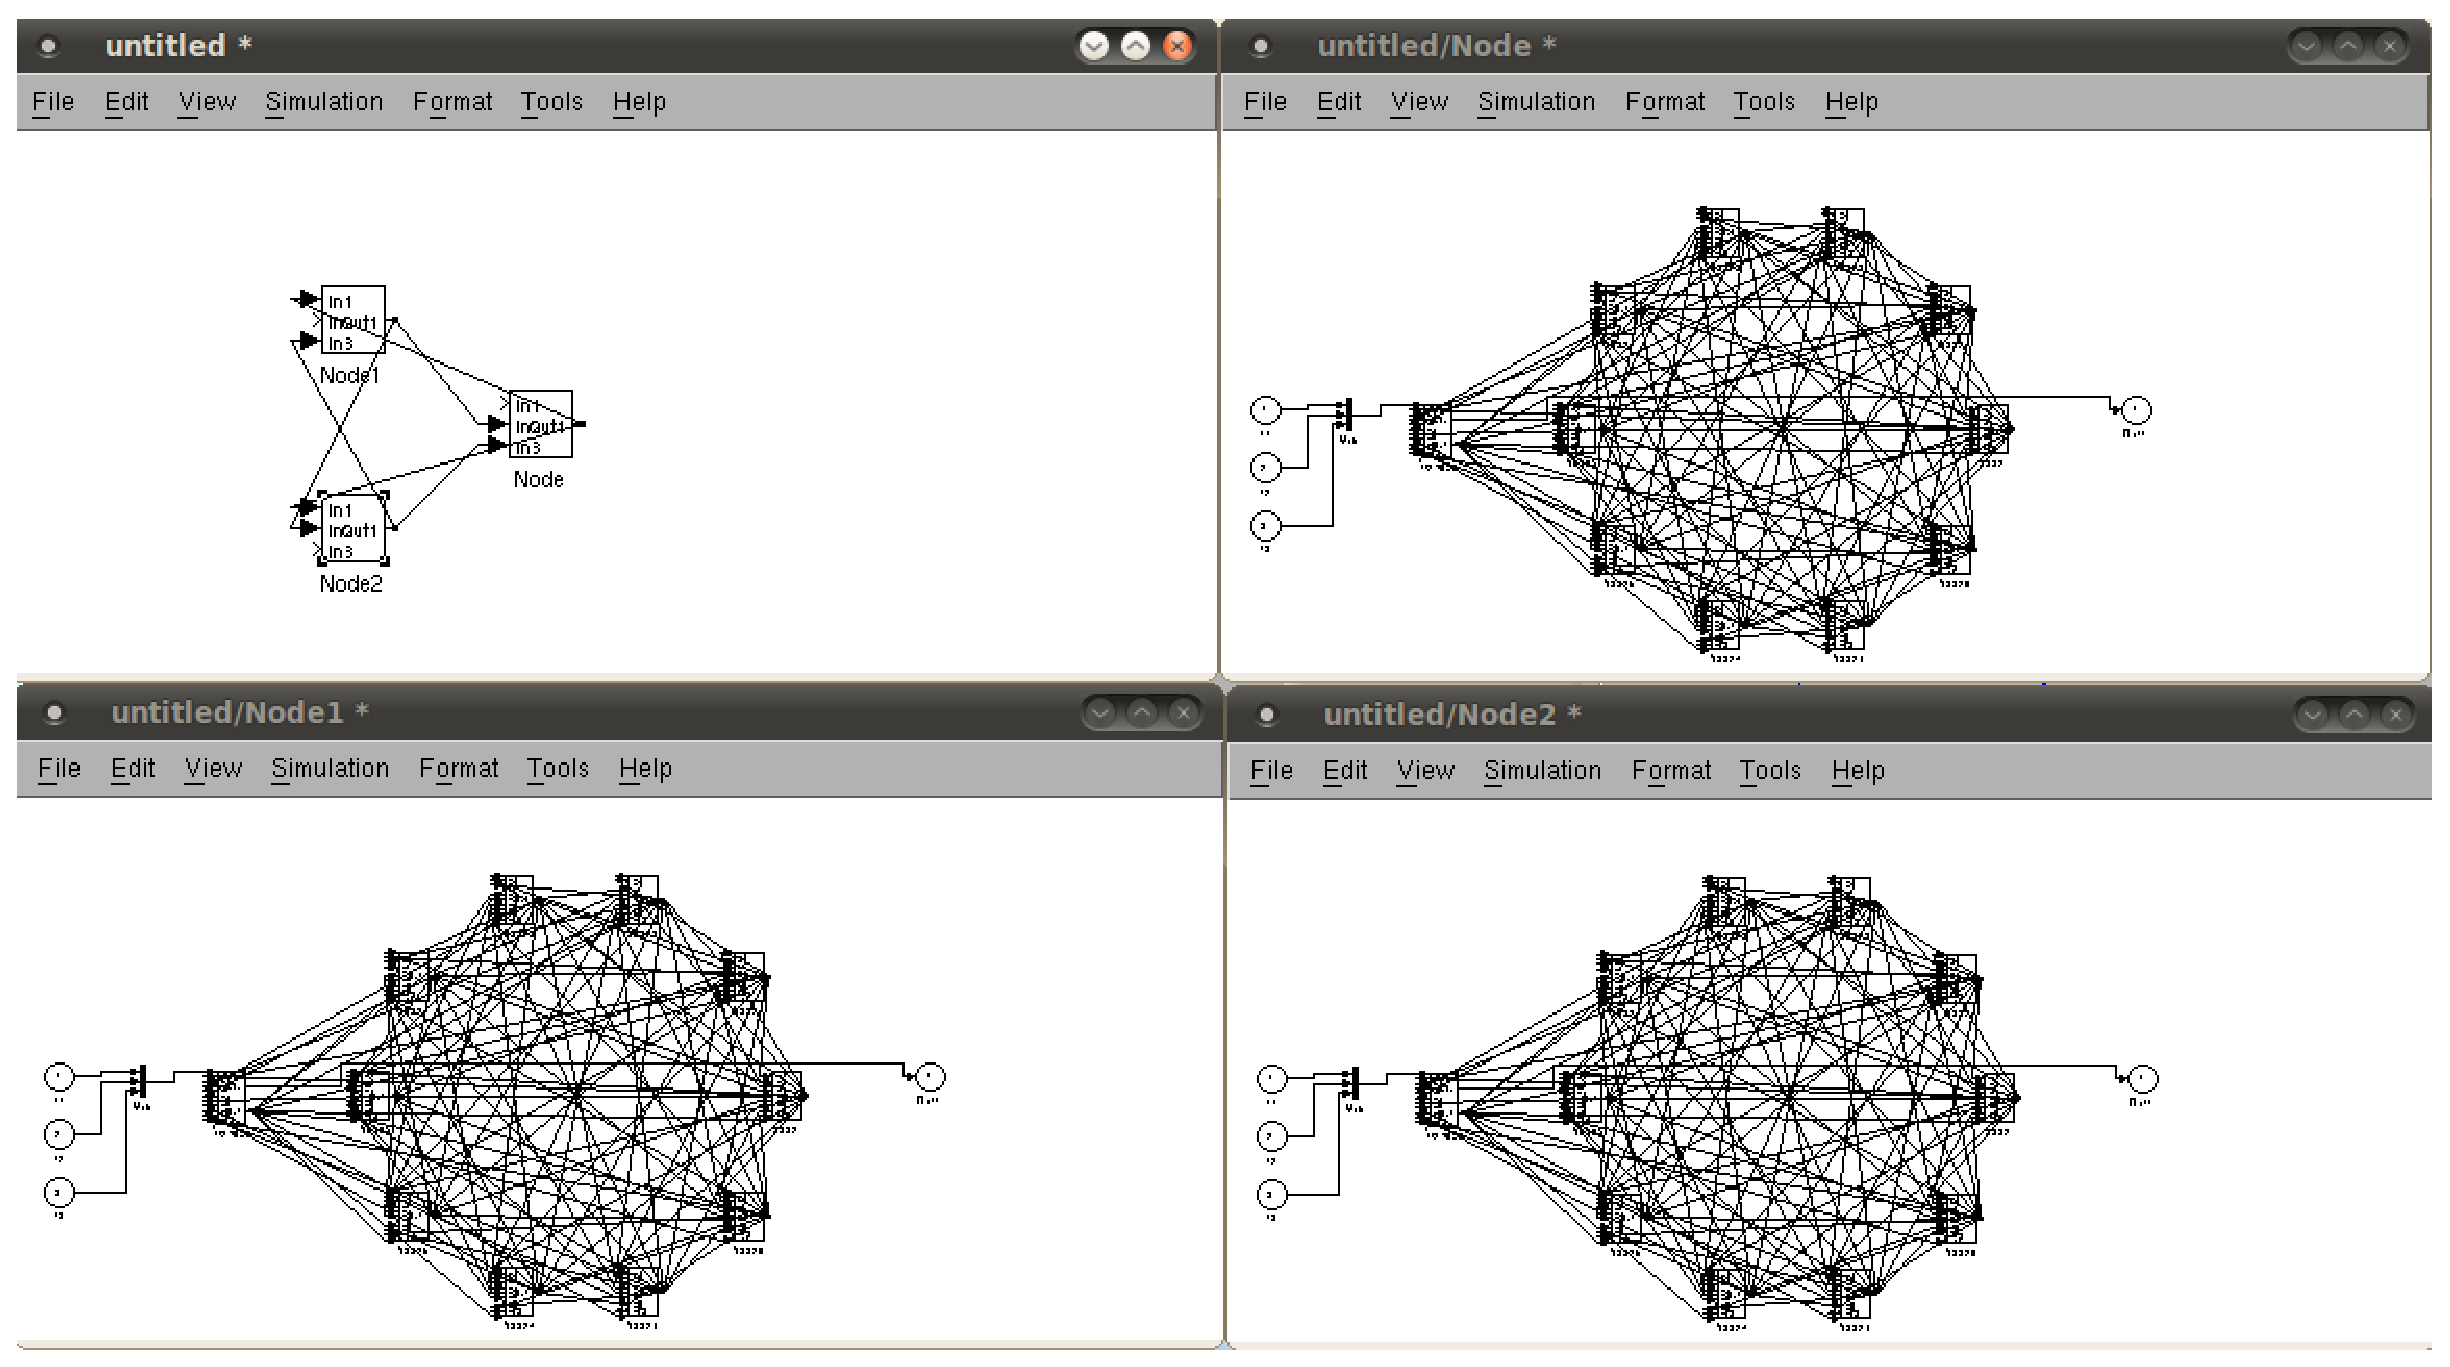
\includegraphics[width=0.5\textwidth]{pics/screenLayers.eps}
\caption[MTIDS model of layered/clustered interconnected systems]{Resulting model of layered/clustered interconnected systems. Example uses a complete graph of 3 nodes where each node is an interface/cluster of a complete graph with 10 LTI nodes plus 1 interface node.}
\label{layersFig}
\end{figure}




\subsection{Build your own Interface Node}

The user may define your own interface node template using the interface node scratch template (\textbf{interfaceTemplate.mdl}). \\

\begin{figure}[htb]
\centering
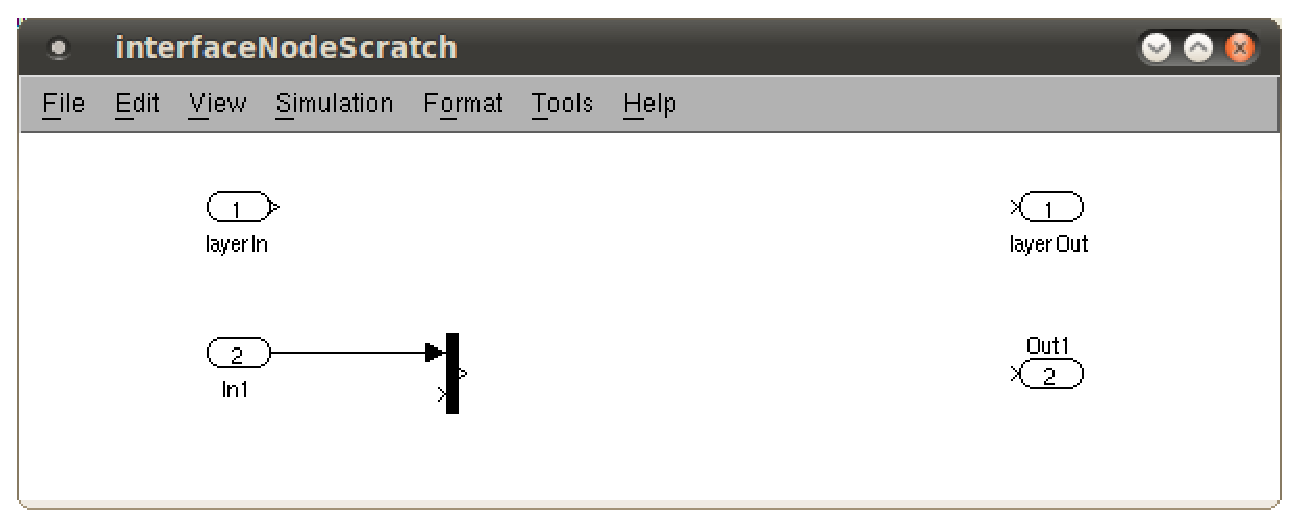
\includegraphics[width=0.5\textwidth]{pics/interfaceTemplate.eps}
\caption[MTIDS interface node scratch template]{Interface node, scratch template model : \textbf{interfaceTemplate.mdl}.}
\label{interfaceFig}
\end{figure}
 
As we see in Figure \ref{interfaceFig} the interface node requires a layer in and out port numbered as $1$, which interacts with other layers/clusters. 
Moreover it requires the basic components of a node template (an in-port connected to a mux and an out-port) in order to interact with the nodes in the cluster/layer.
MTIDS also comes preloaded with a simple aggregating interface template called \textbf{layerInterface.mdl} found under \textbf{/templates}.
 


 

\section{Working in Simulink}\label{workinginsimulink}

Here we review a couple of basic concepts which you will need to run and analyze the simulation of the interconnected dynamic 
systems produced by MTIDS. This is only a quick overview, for more detail please go to : \href{http://www.mathworks.com/help/toolbox/simulink/simulink_product_page.html}{Mathworks Online Simulink Tutorial} or \cite{MatlabBuch}.

\subsection{Simulation Parameters}
The parameters of your model can be defined in Simulink by hand. However, a better way is to 
define the parameters in the Simulink model as variables and give a value to this variables in the Matlab workspace. This also allows you to save this parameters
by saving the workspace as a mat file with the command: \texttt{>> save name.mat}

\subsection{Solver} \label{solver}
Before running a simulation you need to define the simulation runtime and the numerical solver that Simulink will use to simulate your model.
In Simulink: Simulation $\rightarrow$ Configure Parameters, and then going to the solver tab, you may define different types of solver, see Figure \ref{simulink1Fig}.

\begin{figure}[htb]
\centering
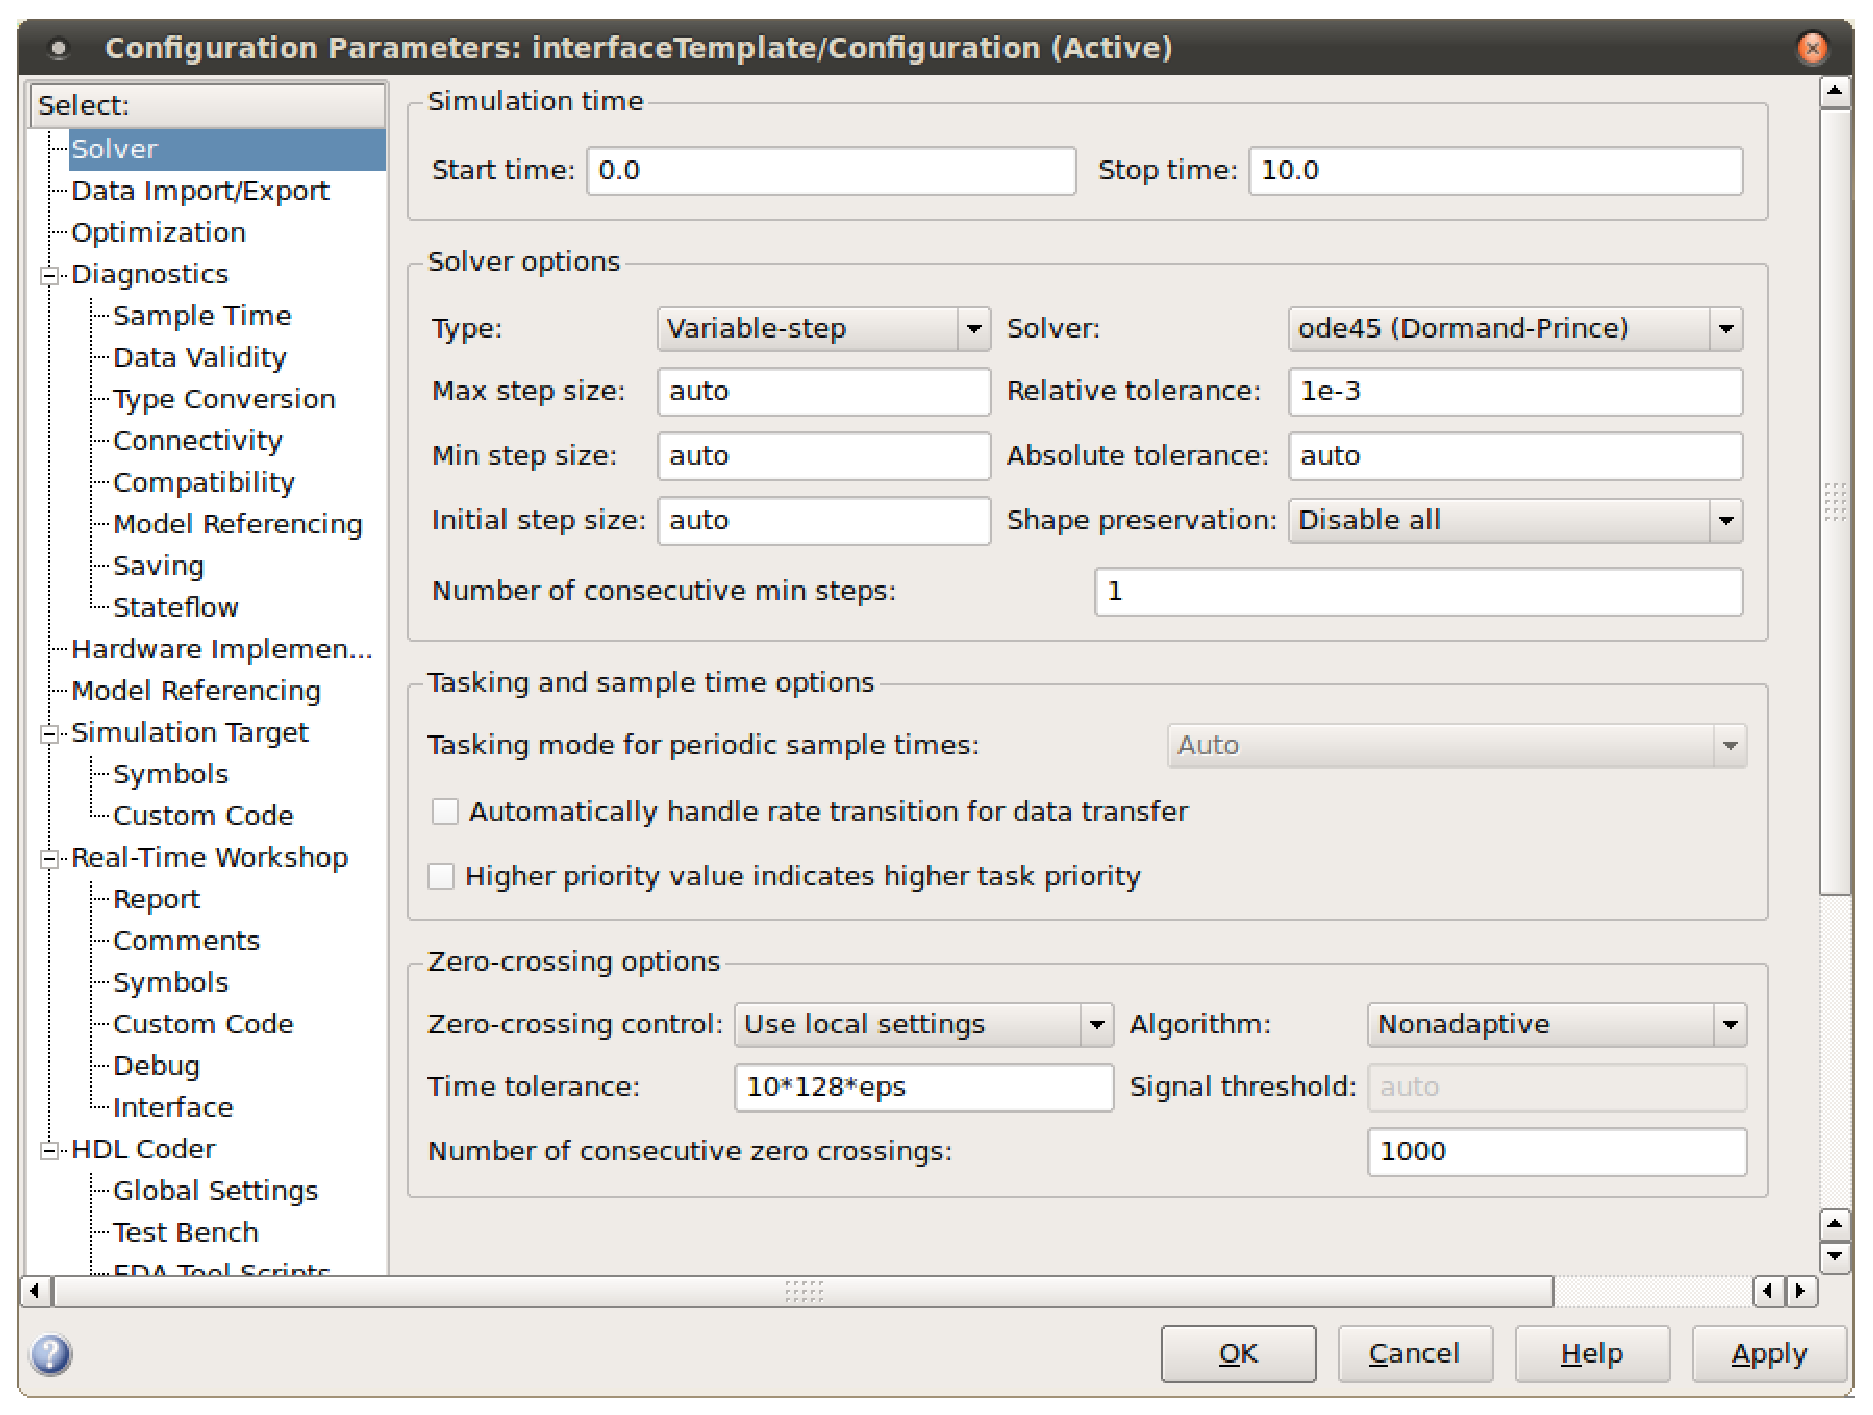
\includegraphics[width=0.5\textwidth]{pics/screenSim1.eps}
\caption[Simulink define solver]{Simulink define solver}
\label{simulink1Fig}
\end{figure} 

It is important to notice that if you want a correct time scale during simulation runtime, you need to define a fixed step size. This is used for the demo of fireflies
synchronization to see the blinking of fireflies in the correct time scale.

\subsection{Visualize Simulation Data}

The easiest way to visualize data during simulations in Simulink is to use scope blocks. The data can then be seen in real-time during simulation.
Another way to do this in real-time, is to use the 'To File' block or the 'To Workspace' block, which allow a direct interaction with Matlab. Plotting functions can be defined in Matlab to interact with the simulation
to show the data in real-time.
\\

The other option is to visualize the results after the simulation. For this, you can define in Simulink which data should be send to the workspace under:
Simulation $\rightarrow$ Configure Parameters in the tab of Import/Export, see Figure \ref{simulink2Fig}. Here, it is useful to export the states, which Simulink defines as the 
values coming out of integrator blocks, but it is also possible to define them by hand.

\begin{figure}[htb]
\centering
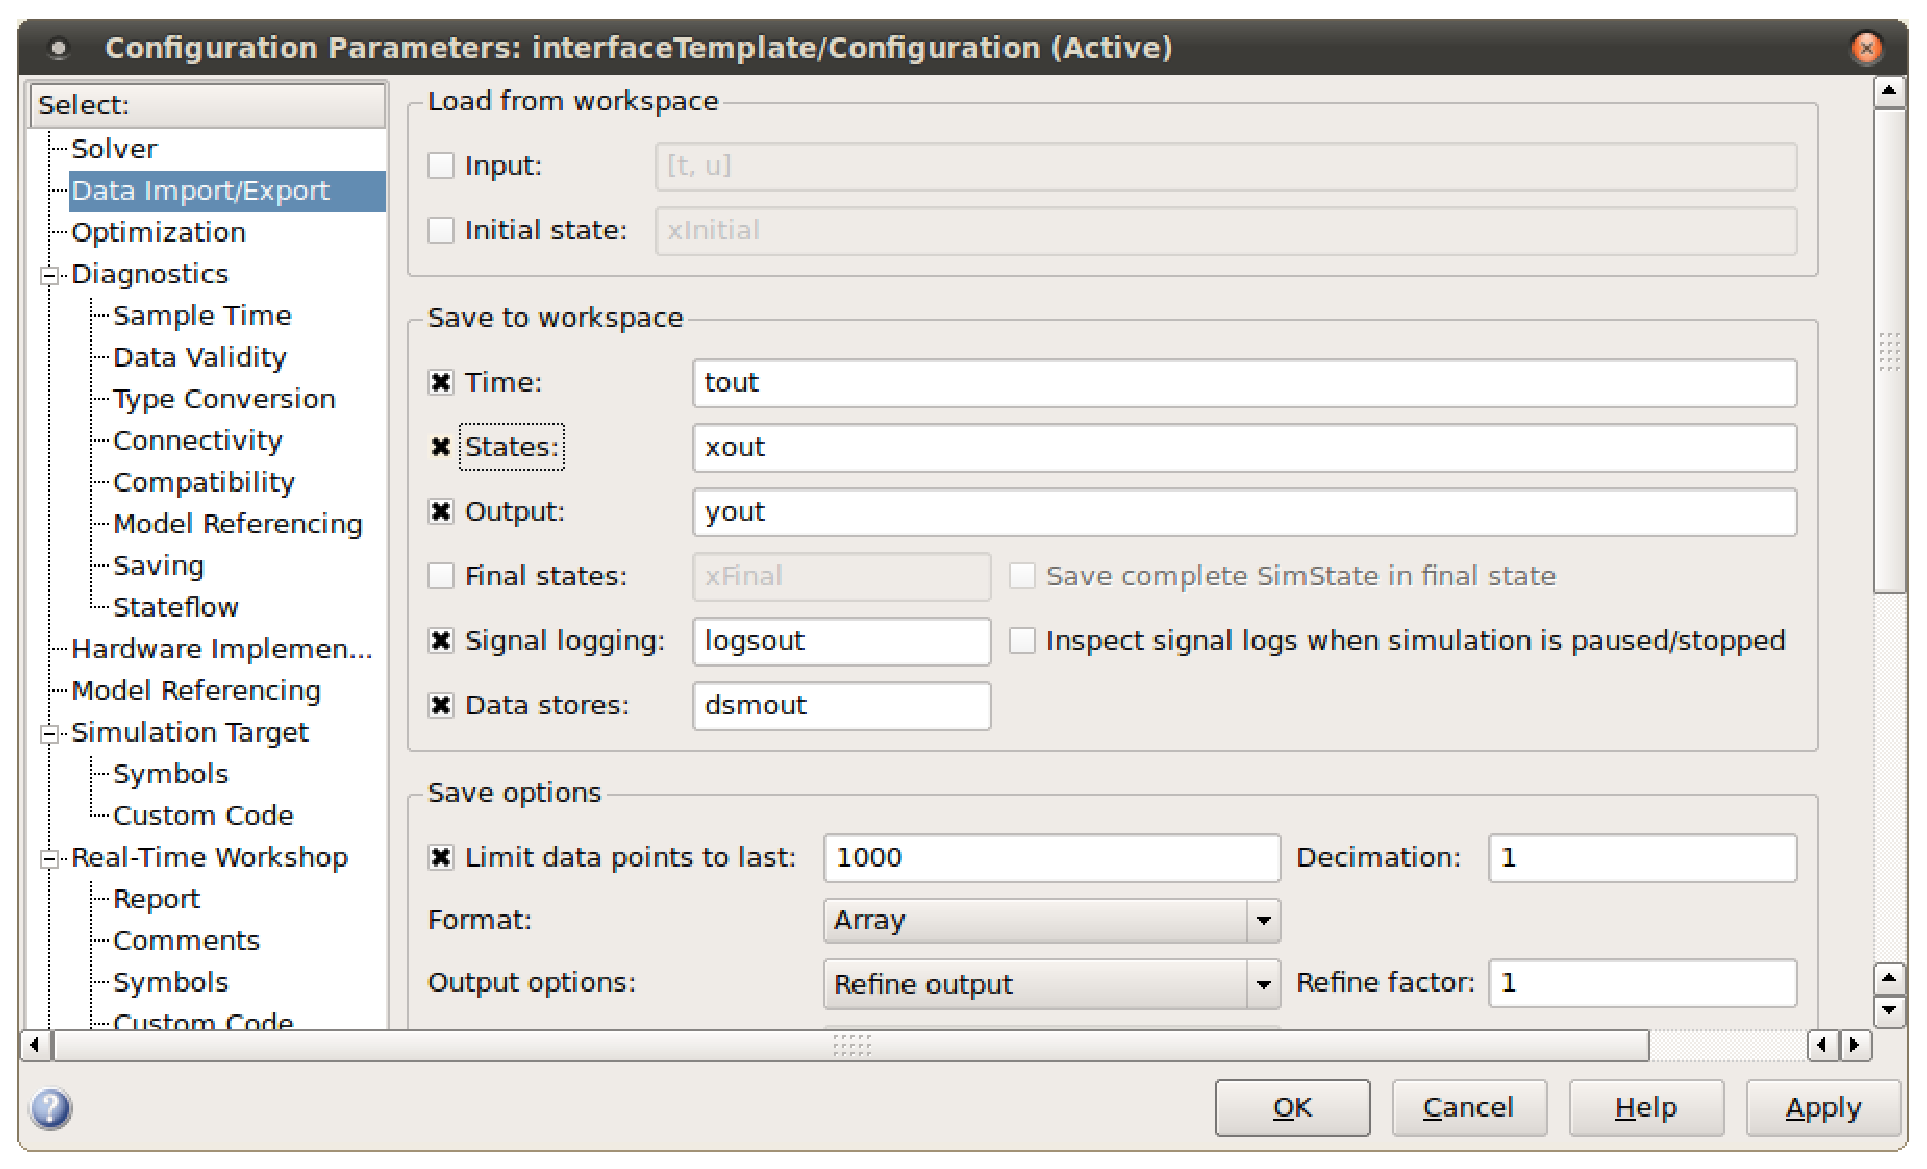
\includegraphics[width=0.5\textwidth]{pics/screenSim2.eps}
\caption[Simulink define import/export data]{Simulink define import/export data}
\label{simulink2Fig}
\end{figure} 

\subsection{Working with a closed Model}

Simulations can also be run from Matlab without the need to open the Simulink model. This is particularly useful for large Simulink models, like models of over 100 nodes that
you may produce with MTIDS. You can write a Matlab script to parametrize  and run the simulation. \textbf{Examples} can be found on the \textbf{help for the \texttt{sim} command}.
% 
% \begin{verbatim}
% Simulate the model, vdp, in Rapid Accelerator mode for an absolute tolerance 
% of 1e-5 and save the states in xoutNew and the output in youtNew.
% 
%    1. Specify parameter name-value pairs within the sim command:
% 
%       simOut = sim('vdp','SimulationMode','rapid','AbsTol','1e-5',...
%                   'SaveState','on','StateSaveName','xoutNew',...
%                   'SaveOutput','on','OutputSaveName','youtNew');
% 
%    2. Specify parameter values in a structure, paramNameValStruct:
% 
%       paramNameValStruct.SimulationMode = 'rapid';
%       paramNameValStruct.AbsTol         = '1e-5';
%       paramNameValStruct.SaveState      = 'on';
%       paramNameValStruct.StateSaveName  = 'xoutNew';
%       paramNameValStruct.SaveOutput     = 'on';
%       paramNameValStruct.OutputSaveName = 'youtNew';
%       simOut = sim('vdp',paramNameValStruct);
% 
%    3. Specify a configuration set containing the parameter values:
% 
%       mdl = 'vdp';
%       load_system(mdl)
%       simMode = get_param(mdl, 'SimulationMode');
%       set_param(mdl, 'SimulationMode', 'rapid')
%       cs = getActiveConfigSet(mdl);
%       mdl_cs = cs.copy;
%       set_param(mdl_cs,'AbsTol','1e-5',...
%                'SaveState','on','StateSaveName','xoutNew',...
%                'SaveOutput','on','OutputSaveName','youtNew')
%       simOut = sim(mdl, mdl_cs);
%       set_param(mdl, 'SimulationMode', simMode)
% \end{verbatim}
% 
% 

 


\section{Import from Simulink}

MTIDS also offers the possibility of importing Simulink models which were produced by MTIDS or are constructed following the MTIDS format, 
see section \ref{subsystemConcept}.\\

\textbf{Notice that the dynamic of the imported system nodes will be the one that you have selected in the MTIDS GUI.}
\\

Node labels, position and topology of the subsytems are imported from Simulink to MTIDS.
To do this in MTIDS: \textbf{Simulation $\rightarrow$ Import from Simulink }, see Figure \ref{mtidsImportFig}. Finally, select the model you wish to import.

Sometimes the nodes are imported in a different order, to correct this click on the \textbf{Circular Visualization} button. 

\begin{figure}[htb]
\centering
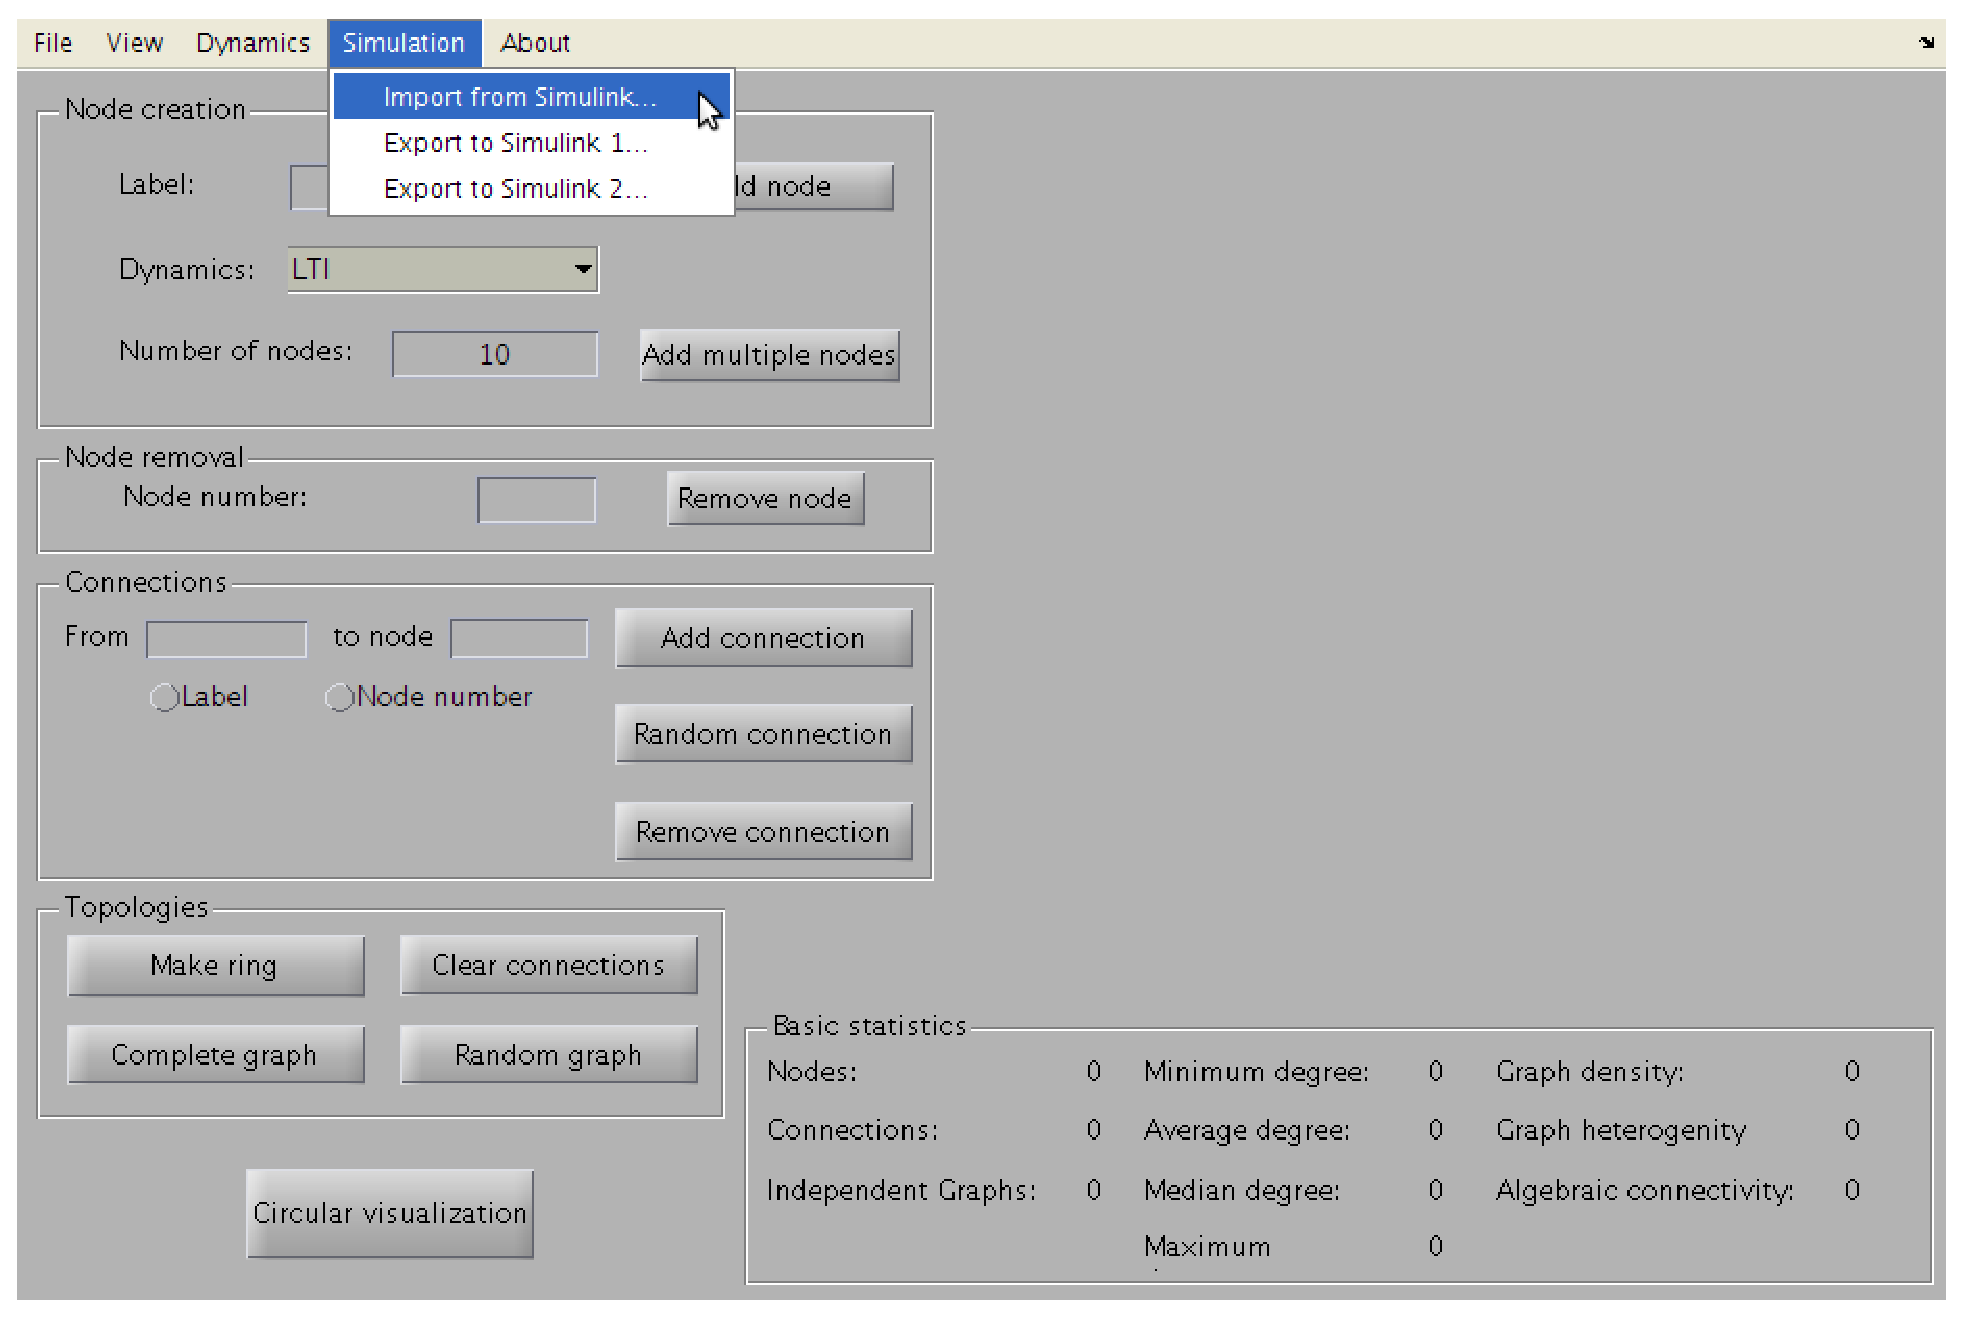
\includegraphics[width=\textwidth]{pics/mtidsImport.eps}
\caption[MTIDS import from Simulink]{MTIDS import from Simulink}
\label{mtidsImportFig}
\end{figure} 

\chapter{Future Development and Conclusion}


\section{Future Development}

MTIDS is a toolbox aimed for students and researchers working in the field of large-scale and interconnected dynamical systems. 
We aim to make this a free and open source tool which can be accessed and improved by the open-source software community in order to
 push research on the field of networked control system forward.\\

There are still some issues and functions which will improve or be implemented in MTIDS:
\begin{itemize}
 \item Support for full import from Simulink.
 \item Support for switching and random interconnections.
 \item Export to Simulink ``wizzard``.
 \item Support for directed graphs.
 \item GUI for interaction with the Control Toolbox.
\end{itemize}
\vspace{5cm} 
\pagebreak 

\section{Conclusion}
In this project we developed a fully functioning toolbox which allows for visual creation and simulation of inteconnected dynamical systems.
MTIDS (Matlab Toolbox of Interconnected Dynamical Systems) is a wrapper that combines tools used for graph theory analysis (Matgraph) and 
for the simulation of interconnected systems (Simulink) to create a flexible and extensible framework.
\\

As MTIDS is based on standard tools used by academia and industry, the User doesn't have to leave the familiar and well documented enviroment of Matlab.
\\ MTIDS capabilities allow for fast setups which makes it an excelent tool for demonstrations (for example in courses on networked control systems),
rapid prototyping for networked and distributed controller design and many more uses.
\linebreak
\newline  
MTIDS features summed up:
\begin{itemize}
 \item Full integration with Matlab and Simulink for simulation and analysis.
 \item Easy Drag and Drop visual system building and connection.
 \item Visualization of key graph properties. 
 \item Nonlinear and switching behavior possible at node level.
 \item Highly customizable thanks to templates.
 \item Layering and clustering capabilities.
 \item Extensible.
\end{itemize}
\smallskip 
MTIDS is available at:
\begin{center}
\textbf{ \href{http://code.google.com/p/mtids/}{http://code.google.com/p/mtids/}}
\end{center}


%
%_______________________________________________________________


%_____Abbildungsverzeichnis_________________________________
\cleardoublepage
\addcontentsline{toc}{chapter}{List of Figures} 
\listoffigures 	 %Abbildungsverzeichnis

%___________________________________________________________
% 
% %_____Literaturverzeichnis_________________________________
 \cleardoublepage
 \addcontentsline{toc}{chapter}{Bibliography}
 \bibliography{mtids_bibliography.bib}
 \bibliographystyle{alpha}
% %__________________________________________________________


%________________Appendix_____________________________________________%


\end{document}
